
\documentclass[12pt]{article}

\title{Machine Learning Private Equity Returns}

\author{
	Christian Tausch  \\
	AssetMetrix GmbH  \\
	Theresienh\"{o}he 13, D-80339 Munich \\
	christian.tausch@quant-unit.com \\
	\and 
	Marcus Pietz  \\
	AssetMetrix GmbH  \\
	Theresienh\"{o}he 13, D-80339 Munich \\
	marcus.pietz@asset-metrix.com \\
	}

\date{\today}



% Packages
\usepackage{amssymb}
\usepackage{amsmath}
\usepackage{natbib}
\usepackage{graphics}
% use smaller margins
\usepackage[margin=1.1in]{geometry} % 1.25in
\usepackage[margin=1.1cm]{caption}
% use double spacing
\usepackage{setspace}
\usepackage{amsthm}
\usepackage{url}
\usepackage[outdir=./]{epstopdf}
\usepackage{booktabs}
\usepackage{float}
\usepackage{standalone}
\usepackage{xcolor}


\newtheorem{prop}{Proposition}
\newtheorem{assume}{Assumption}

\definecolor{darkgreen}{rgb}{0.0, 0.5, 0.0}


% logo
\usepackage{fancyhdr}
\usepackage{graphicx }

\iffalse
%\addtolength{\headheight}{1cm} % make more space for the header
\pagestyle{fancyplain} % use fancy for all pages except chapter start
\lhead{
\includegraphics[height=0.6cm]{logo/quantunitcom}} % left logo
\rhead{
\includegraphics[height=0.6cm]{logo/AssetMetrixLogo2019schwarz}} % right logo
%\renewcommand{\headrulewidth}{0pt} % remove rule below header
\renewcommand{\chaptermark}[1]{ \markboth{#1}{} }
\renewcommand{\sectionmark}[1]{ \markright{#1}{} }
\fi


\begin{document}

\maketitle


\section*{Keywords}
Return factor model,
Private equity, 
Public factor exposure, 
Model combination, 
Machine learning,
Ensemble learning


\section*{Acknowledgements}
We thank Nicolas D\"{u}tsch, Philipp Abel, and Kai Urban for valuable feedback and helpful comments that greatly improved the paper.


\section*{Declaration of interest}
The authors report no conflict of interest. 
The authors alone are responsible for the content and writing of the paper.


\newpage
%\doublespacing

\begin{center} 
\section*{Machine Learning Private Equity Returns}
\end{center}



\abstract{
	In this paper, we use two machine learning techniques to learn the aggregated return time series of complete private capital fund segments.
	First, we propose Stochastic Discount Factor (SDF) model combination to determine the public factor exposure of private equity.
	Here, we describe our theoretical motivation to favor model combination over model selection.
	This entails that we apply simple coefficient averaging to obtain multivariate SDF models that mimic the factor exposure of all major private capital fund types.
	As a second step, we suggest componentwise $L_2$ boosting to estimate the error term time series associated with our factor models.
	The simple addition of the public factor model returns and the error terms then yields the total return time series.
	These return time series can be applied for proper integrated public and private risk management or benchmarking.
}


\section{Introduction}
\label{sec:factor_investing}

Factor investing has gained widespread popularity in public markets due to its ability to discern the underlying drivers of returns. 
Articulating a portfolio's exposure to public factors entails a comprehensive understanding of both its realized returns and the expectations for future risk and return. 
For private market investors, meaningful insights can be derived from realistic factor decompositions, presuming the existence of shared components influencing both public and private returns. 
In light of this perspective, our factor analysis dissects private equity returns into a traded return component and its corresponding error terms. 
The primary applications of our return decomposition extend to public market equivalent benchmarking, comprehensive risk management, and strategic asset allocation.

Generally, more sophisticated methods are required to estimate factor models for private (in comparison to public) asset classes as private returns are not directly observable on liquid secondary markets.
However, the challenge of identifying the 'best' factor model is the same as in public markets.
There are first attempts to select or create public indices that shall replicate private equity (PE) returns.
Here, we can distinguish between (i) factor- and (ii) holding-based approaches.
\cite{P14} benchmarks buyout funds against several factor indices.
More subtle factor-based methods are mainly established in the hedge fund replication literature \citep{TV08,W14}.
To avoid overfitting, \cite{OST17} propose to combine multiple factor models for passive hedge fund replication.
Holding-based approaches to mimic the PE investment style are proposed by \cite{LSSL16}, \cite{S17}, \cite{MS19}, and \cite{PP19}.
This paper pursues a factor-based solution that employs publicly traded indices and does not require deal-level information on PE funds.
In contrast to the factor-based ansatz of \cite{P14}, we base our approach on 
\textcolor{darkgreen}{Stochastic Discount Factor} 
(SDF) models that are estimated on PE fund-level data rather than comparing several ad-hoc choices for potentially suitable indices.

This article aims at a data-science-driven solution to describe PE returns.\footnote{See \cite{CG23} for a textbook treatment of machine learning methods for factor investing.}
Concretely, we propose SDF model combination (of factor models estimated by the \cite{DLP12} method) as a straightforward method to obtain 'strong' public factor models that explain private equity returns.
Here, we provisionally define the term 'strong' versus 'weak' model in analogy to the boosting literature \citep{S90}.
A 'strong' model shall exhibit small (error term) bias and variance, whereas a 'weak' model displays high bias and variance.
Only the 'true' or 'best' or 'optimal' model obtains an error term of precisely zero.

As we cannot expect a perfect model with zero error terms in any realistic setting, we try to explicitly model these error terms by means of machine learning.
Usually, estimation procedures for linear return factor models like $R_t= \alpha + \beta^{\top} X_t + e_t$ are mainly interested in estimating the factor loadings $\beta$ and the constant outperformance term $\alpha$.
For private equity fund returns only \cite{ACGP18} propose a Markov Chain Monte Carlo (MCMC) approach to estimate also the error terms $e$.
As an alternative to their method, our paper suggests a statistical learning technique called componentwise $L_2$ boosting to estimate the error term time series belonging to a given public factor model.
Moreover, in stark contrast to \cite{ACGP18}, our model does not assume a parametric distribution for the error term $e$.
Figure \ref{fig:how} illustrates our general machine learning approach to derive the public and private part of private equity returns.

The paper is structured as follows.
Section \ref{sec:semiparametric_setting} introduces the method's underlying semiparametric setting.
Section \ref{sec:model_selection} explains why model selection is problematic.
Section \ref{sec:model_combination} introduces two estimation procedures: model combination for the public factor model and componentwise $L_2$ boosting for the error terms.
Section \ref{sec:applications} successfully applies the estimation procedures to a real-world dataset.
Section \ref{sec:conclusion} concludes.
%Moreover, appendices \ref{sec:vc_errors} until \ref{sec:errors_pd} outline the error term time series for several private capital fund segments. 
%Appendix \ref{sec:pitchbook} gives further information on the Pitchbook dataset used for empirical estimation.
%Appendix \ref{sec:preqin} gives model results based on Preqin data (instead of Pitchbook data).
Finally, the \texttt{R} code used for model estimation can be found in the following online repository \url{https://github.com/quant-unit/Fundwise_SDF}.

\begin{figure}[ht]
	\centering
	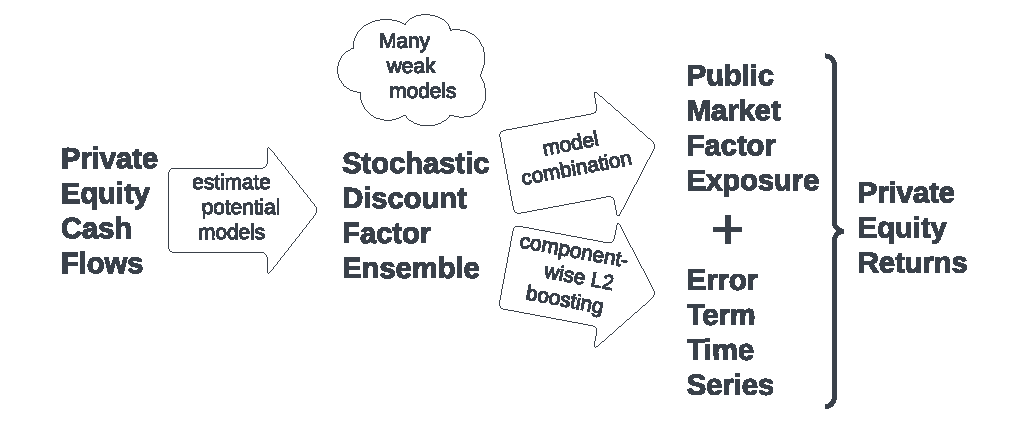
\includegraphics[width=14cm]{FlowChart/MLPER}
	\caption{How to translate private equity cash flows to private equity returns?}
	\label{fig:how}
\end{figure}

\section{Semiparametric setting}
\label{sec:semiparametric_setting}

Stochastic Discount Factors (SDFs) are econometric models to price a given cash flow stream \citep{HR87}.
They are usually estimated by semiparametric approaches that go without a parametric model for the error term \citep{F19}.
Following \cite{DLP12}, the cash flows stream under consideration is generated by $i=1,2,\dots,n$ private equity funds (or portfolios).
SDFs can be applied in net present value calculations for realized cash flow paths
\begin{equation}
\label{eq:pricing_error}
P_{\tau, i} =
\sum_{t=1}^{T}\ \Psi_{\tau, t}\ {CF}_{t, i}
\end{equation}
with price $P$, SDF functional $\Psi$, and cash flow stream $CF$. 
Time is discrete with $t=1,2,\dots,T$.
If the 'true' SDF model is applied, the expected price $\mathbb{E}[P]=0$.\footnote{We also refer to $P$ as pricing error since we want to avoid any average price deviation from zero, i.e., minimize the expected pricing error.}
Thus the functional form and explanatory variables used in the 'true' SDF explain or describe the risk and return properties of the cash flows. 
Further, if we have an appropriate SDF for a given private equity fund type, we can apply it in a simple net present value calculation (as in the formula above) to assess the outperformance of a specific private equity fund. 
A positive/negative net present value indicates an out/under-performance compared to other PE funds.
To discount a time $t$ cash flow to time $\tau$, we use the simple linear multi-period SDF model
\begin{equation}
\label{eq:linear_sdf}
\Psi_{\tau,t} =
\frac{
	\prod_{h=0}^{\tau}\ \left(1 + \alpha + r_{h} + \sum_j\ \beta_j\ F_{j,h} + e_h \right)
}{
	\prod_{h=0}^{t}\ \left(1+ \alpha + r_{h} + \sum_j\ \beta_j\ F_{j,h} + e_h \right)
}
\end{equation}
with usually $\alpha=0$, $e_h=0 \ \forall \ h$, risk-free rate $r$, zero-net-investment factor return $F$, and factor coefficient $\beta$ that has to be estimated from data. 
Consequently, the expected multi-period return for a given asset is modeled by
\[
E \left[R_{\tau,t} \right] = 
E \left[ \frac{1}{\Psi_{\tau,t}} + \epsilon_{\tau,t} \right]
\]
where the period-specific error term $\epsilon_{\tau,t}$ has zero expectation $E[\epsilon_{\tau,t}]=0$.

As commonly seen in the asset pricing literature, we estimate SDF model coefficients by semiparametric approaches that require no distributional assumption for $\epsilon_{\tau,t}$.
This means we select $\alpha$ and $\beta$ values that yield average pricing errors close to zero. 
Here the typical loss function choices are quadratic forms like in Generalized Method of Moments (GMM) or a quadratic or least absolute deviance loss function $L()$
\begin{equation}
\label{eq:minimization_estimation}
\hat{\theta } = \
\arg \min_{\theta} \frac{1}{n} \sum_{i=1}^n L \left( P ; \theta, \gamma \right)
\end{equation}
where $\theta=(\alpha,\beta)$ and $\gamma$ denotes the vector of potential hyperparameters like data cutoff dates or weighting/averaging methods.
More details on the semiparametric estimation framework can be found in the original paper of \cite{DLP12} and its credit market factor application by \cite{HSS23}.
As a little modification of their native method, we average over multiple compounding dates $\tau \in \mathcal{T}$ in our quadratic loss function
\begin{equation}
	\label{eq:quadratic_loss}
	L \left( P ; \theta, \gamma \right) = \left( \frac{1}{|\mathcal{T}|} \sum_{\tau \in \mathcal{T}} P_{\tau,i}  \right)^2
\end{equation}
to decrease the small-sample bias and variance of the estimator.


\section{So many weak SDF model candidates}
\label{sec:model_selection}

In the semiparametric setting described in section \ref{sec:semiparametric_setting}, we likely obtain many weak model candidates with no clear winner among them.
This scenario is comparable to the extensive ``factor model zoo'' observed in public equity markets, as coined by \cite{C11,FGX20}. Furthermore, the extensive body of public market literature fails to definitively determine which factors provide the most comprehensive explanation for their assets' returns.
In this section, we explain in greater detail why we also expect to be confronted with (i) many but (ii) weak SDF model candidates in the private equity case.
Moreover, we discuss why it is challenging to select the single 'best' model from an extensive collection of homogeneous competitors (that all use the same SDF model as specified in equation \ref{eq:linear_sdf}).

\subsection{Why are there so many models?}

First, there exists a great variety of different public return factor candidates that might be also relevant for private equity. 
It is not even clear which factors 'best' explain public equity returns, cf. references in \cite{KN20}. 

Second, we can choose from many feasible semiparametric estimators, loss functions, or ancillary machine learning methods, cf.\ \cite{GKX20} for a public market overview.
Additionally, there are discretionary choices for regularization- or other hyperparameters.
Further, bootstrapping and other resampling-based techniques may be helpful but likewise dramatically increase the number of model candidates.

Third, in contrast to common public databases available for public equity, the private equity literature has to draw on various private -- often proprietary -- data sources. 
When estimating the same model on different datasets, the coefficient estimates will differ. 
Unclear data cutoff dates or horizons exacerbate this issue.

\subsection{Why are the models so weak?}

First, private equity data is notoriously sparse as the first PE funds were established in the 1970s to 80s.
Moreover, it is currently (almost) impossible to collect data on all funds from a given vintage. 
These issues render finite [infinite] sample inference more [less] reliable.

Second, for fund-level data, the dependency issue introduced by overlapping fund cash flows further reduces the number of truly independent observations. 
Similarly, financial engineering applied on fund level like bridge financing or Net Asset Value (NAV) facilities undermine the explanatory power of observed fund cash flows.

Third, in private equity, limited sample sizes typically allow the inclusion of just 1-2 factors in a SDF model; 
even many two-factor models appear to be statistically insignificant (weak models); 
models with more covariates almost surely overfit (invalid models).


\subsection{Why is model selection difficult?}

First, model uncertainty is particularly high for weak models, as we cannot be sure which single model performs best when we test several competing models/factors.

Second, as there are many model candidates but limited data, data snooping may be a general problem \citep{W00}. 

Third,  correct inference post model selection is essential but known to be challenging \citep{BLP19}. 
This means classical statistical inference results only apply for testing a single model. 
When we want to compare several model candidates, the application of these basic statistical methods yields invalid inference results.


\section{And the jury selects: model combination}
\label{sec:model_combination}

A powerful alternative to model selection is model combination.
Generally, Bayesian and frequentist model averaging is a well-studied field in classical statistics \citep{H14,M15}.
Similarly, ensemble learning, a prominent subfield of machine learning, builds on the notion to form a strong learner by combining many weak learners \citep{B12}.
In more applied settings, predictive forecast combination often helps to increase forecast precision \citep{HL10}.
In a public market setting, \cite{RSZ10} forecast the public equity premium by combining 15 univariate OLS regressions of different macroeconomic predictors.
Probably most closely related to our case, \cite{OST17} advertise model combination for passive hedge fund replication.


\subsection{Model averaging}
\label{sec:model_averaging}

As we potentially want to exclude invalid models from combination, the set of valid models is defined as the $M^*$ models with the smallest absolute pricing error $M^*=\{m \in M: P^{(m)} \leq Q(x;P) \}$ where $Q$ is the pricing error quantile function and quantile value $x = \frac{M^*}{M}$.
Here, $M$ is the number of all valid and invalid SDF models.
Generally, we can also apply more sophisticated -- but also more time-consuming -- cross-validation procedures \citep{AC10} 
\textcolor{darkgreen}{or the Model Confidence Set approach of \cite{HLN11}} 
to distinguish between valid and invalid models.
The simpler alternative is to assume that all SDF models estimated by the researcher are valid, i.e. $M^*=M$ with $x=1$.
Finally, the weighted pricing error obtained by SDF model averaging is defined as
\begin{equation}
\label{eq:model_averaging}
\mathcal{E}_{\tau, i}^{(M^*)} = 
\sum_{m=1}^{M^*} \  
w_m \
\sum_{t=1}^{T} \
\Psi_{\tau,t}^{(m)}\ 
{CF}_{t, i}
\end{equation}
with model weight $w_m \geq 0$ and all weights sum to one $\sum_m^{M^*}\ w_m=1$. 
If a similar predictive performance for all valid models can be assumed, equal weighting $w=(M^*)^{-1}$ is advised.\footnote{The forecast combination puzzle states that simple equal-weighting practically often performs better than more complex (theoretically optimal) combination schemes \citep{SW09,CMVW16,QRCY19}.}.
Otherwise, we shall overweight more predictive models with smaller pricing errors, e.g., the weight may be proportional to the inverse of the absolute pricing error $\left(\left|P\right|\right)^{-1}$.

\subsection{Coefficient averaging}
\label{sec:coef_averaging}

The general model combination approach defined by equation \ref{eq:model_averaging} allows the aggregation of structurally distinct SDF models.
If we always employ the same linear SDF as defined in equation \ref{eq:linear_sdf}, which can be replicated by an investable trading strategy, model combination can be interpreted as a diversification strategy.
The idea is to invest in several promising strategies rather than committing entirely to a single ``optimal'' trading strategy.
Using always the same linear SDF model enables the following coefficient averaging formula, which only approximates the diversified pricing error from equation \ref{eq:model_averaging} (the better when the factor returns -- thus return horizons -- are small).
\begin{equation}
\label{eq:coef_averaging}
\beta_j^{(M^*)}\ =\ \sum_{m=1}^{M^*}\ w_m \ \beta_{j,m}
\end{equation}
The idea here is that one multivariate model that includes all traded factors can be better perceived and interpreted as an ensemble of $M^*$ heterogeneous one- or two-factor models.

Finally, with the $\beta_j^{(M^*)}$ coefficient estimated, we can focus on the $\alpha$ term in equation \ref{eq:linear_sdf}.
To quantify the public market out/underperformance, we can apply the Excess-IRR method described by \cite{PG09}, which estimates the $\alpha$ term by setting the pricing error to precisely zero for each $i$
\begin{equation}
	\label{eq:exess_irr}
\hat{\alpha}_i = \arg \min_{\alpha_i} \left| P_{\tau, i}^{(M^*)}  \right|
\end{equation}
Alternatively, we can directly calculate the Internal Rate of Return (IRR) associated with the SDF discounted cash flows (with $\alpha=0$ in equation \ref{eq:linear_sdf}), which corresponds to the direct-alpha method described by \cite{GGS23}.
In both cases, we estimate the constant out/underperformance term for the $i$th portfolio after adjusting for systematic risk factors.

\subsection{Estimating idiosyncratic returns}
\label{sec:error_term_estimation}

In the spirit of equation \ref{eq:exess_irr}, we can also try to find an estimate for the series $e=(e_h)_{h=1,2,\dots,T}$ from equation \ref{eq:linear_sdf} instead of estimating the constant $\alpha$.
For illustrative purposes, we select here a conceptually simple, but brute-force machine learning algorithm called componentwise $L_2$ boosting \citep{B06}.
In general, we can choose any high-dimensional statistical method that can be used for variable selection like the canonical lasso \citep{BG11}.
In the probably most closely related paper to our problem, \cite{ACGP18} use a Bayesian Markov Chain Monte Carlo (MCMC) method to estimate the systematic and also idiosyncratic return component of private equity returns.

In our approach, we start with a set of $\alpha$ and $\beta$ estimates and learn the idiosyncratic error term time series $e$ conditional on these initial estimates.
Concretely, we estimate in the first step an ensemble of size $M_{\mathrm{systematic}}$ consisting of reasonable estimates for $\alpha$ and $\beta$ by iteratively applying traditional non-linear optimization (using a different set of factors $F$, dataset samples, or hyperparameters $\gamma$ in each iteration).

In the second step, we use componentwise $L_2$ boosting to estimate a new series $e$ for each of the $M_{\mathrm{systematic}}$ public factor ensembles.
Componentwise $L_2$ boosting (CLB), also known as gradient boosting with the $L_2$ loss function, is a machine learning algorithm that belongs to the family of boosting methods. 
Boosting is an ensemble learning technique where weak learners (usually simple models like decision trees) are sequentially trained, and each new learner focuses on correcting the errors made by the existing ensemble.
In the context of boosting, "componentwise" refers to the fact that each weak learner added to the ensemble is trained to fit the residual errors of the existing ensemble. 
This is done in a way that the new learner addresses a specific component of the overall prediction.
The original paper of \citep[Section 2]{B06} gives the exact mathematical definition of the CLB algorithm.
Financial applications of the CLB method can be found in \cite{bai2009boosting}, \cite{mittnik2015stock}, and \cite{tausch2019quadratic}.

In our case, the CLB algorithm can be described by the following "brute-force" iterative procedure. 
We apply these CLB steps to each public factor model (of the previously estimated ensemble of size $M_{\mathrm{systematic}}$) separately.
\begin{enumerate}
	\item \textbf{Initialization:} 
	The boosting process starts with the public factor model without error terms ($e_t = 0 \ \forall \ t$) as initial model. 
	The first weak learner is then trained to minimize the $L_2$ loss on the training data, considering the difference between the true outcomes and the predictions made by the current ensemble (which is the initial factor model).
	\item \textbf{Sequential Training:} 
	In each subsequent iteration, a new weak learner -- in the form of an error vector $e$ update -- is added to the ensemble. 
	This learner is trained to fit the negative gradient of the $L_2$ loss with respect to the current ensemble's predictions. 
	In other words, it focuses on the residuals, the differences between the true outcome (which is a zero pricing error in equation \ref{eq:quadratic_loss}) and the pricing error made by the current ensemble.
	This means that, at each step, the boosting algorithm is effectively optimizing the ensemble by sequentially addressing the weaknesses of the current predictions.
	\item \textbf{Componentwise Correction:} 
	The term "componentwise" emphasizes that each weak learner corrects only one specific component (date) of the overall error time series $e$. 
	Concretely, one boosting step simultaneously optimizes each component of the vector $e$ to reduce the pricing error.
	However, only the component of the $e$ vector (i.e., a single date $t$) that yields the minimal pricing error, when compared to all other optimized $e$ vector components, is used to update the factor model.
	\item \textbf{Shrinkage:} 
	Componentwise $L_2$ boosting often incorporates a shrinkage parameter between zero and one, which controls the contribution of each weak learner to the ensemble (in our empirical example: 0.33). 
	This helps prevent overfitting.
	\item \textbf{Early Stopping:} 
	The steepness of the gradient or cross validation techniques can be employed to determine the optimal stopping time of the algorithm. 
	With too many boosting iterations CLB likely overfits.
	In our empirical example, we stop after 200 boosting steps.
	\item \textbf{Final Prediction:} 
	The final prediction for the error term time series $e$ is the sum of the predictions made by all the weak learners in the error ensemble.
\end{enumerate}

Finally, in the spirit of model combination, we average over the $M_{\mathrm{systematic}}$ estimates of $\alpha$, $\beta$ and $e$ to obtain our final factor model estimates.
Since $\alpha=E[e]$, we can, without loss of generality, set $\alpha=0$ in our estimation procedure.
In practice, it could however be beneficial in some cases to start with a ``good initial guess value" for $\alpha$.


\section{Empirical application}
\label{sec:applications}

\subsection{Factor exposure by fund segment}
\label{sec:factor_exposure}

In this section, we apply our model combination methodology to replicate the factor exposure of PE funds.
The resulting SDF models employ MSCI indices and are estimated by our augmented version of the \cite{DLP12} method.
Specifically, all SDF ensembles draw on (valid) two-factor models, where the first factor is always the MSCI World excess return over the risk-free rate and the second factor is a long-short combination of MSCI World style indices:
\begin{description}
	\item[MKT-RF:]{MSCI Market Return Minus Risk-free Rate}
	\item[SMB:]{MSCI Small Cap Minus MSCI Large Cap Return}
	\item[HML:]{MSCI Value Minus MSCI Growth Return}
	\item[HDY-MKT:]{MSCI High Dividend Yield Minus MSCI Market Return}
	\item[QLT-MKT:]{MSCI Quality Minus MSCI Market Return}
\end{description}
For each of the 4 factors (SMB, HML, HDY-MKT, QLT-MKT), we estimate an ensemble of $2 \times 2 \times 5$ bivariate two-factor models with (i) quadratic and least absolute deviance loss function $L()$, (ii) both equal- and fund-size-weighted cash flows, and (iii) maximum months 120, 150, 180, 210, 240.
\textcolor{darkgreen}{
	As we consider all models to be valid, no model is excluded ($M^*=M$).
}
Next, we use the simple coefficient averaging as described in subsection \ref{sec:coef_averaging} to obtain five-factor models.

% latex table generated in R 4.2.1 by xtable 1.8-4 package
% Wed May 10 16:40:54 2023
\begin{table}[ht]
	\centering
	\begin{tabular}{llllll}
		Type & MKT-RF & HML & SMB & HDY-MKT & QLT-MKT \\ 
		\hline
		\hline
		% ALL & 1.19 (0.2) & -0.16 (0.06) & -0.15 (0.04) & -0.25 (0.09) & -0.1 (0.03) \\ 
		BO & 1.4 (0.15) & -0.1 (0.02) & -0.09 (0.02) & -0.15 (0.03) & -0.1 (0.04) \\ 
		DD & 1.04 (0.25) & 0.25 (0.02) & 0.29 (0.02) & 0.54 (0.07) & 0.01 (0.06) \\ 
		% FOF & 1.14 (0.34) & -0.08 (0.26) & -0.29 (0.08) & -0.52 (0.17) & -0.23 (0.1) \\ 
		INF & 0.71 (0.45) & 0.13 (0.09) & 0.13 (0.04) & 0.22 (0.08) & 0.73 (0.38) \\ 
		MEZZ & 0.75 (0.16) & 0.03 (0.04) & 0.16 (0.07) & 0.14 (0.05) & 0.14 (0.15) \\ 
		NATRES & 0.48 (0.29) & 0.02 (0.15) & 0.06 (0.17) & 0.1 (0.23) & -0.37 (0.09) \\ 
		PD & 0.69 (0.25) & 0.13 (0.05) & 0.19 (0.08) & 0.31 (0.11) & 0.21 (0.14) \\ 
		%PE & 1.31 (0.2) & -0.18 (0.09) & -0.14 (0.06) & -0.25 (0.11) & -0.06 (0.03) \\ 
		RE & 1.05 (0.5) & 0.02 (0.1) & -0.33 (0.07) & -0.43 (0.17) & -0.55 (0.11) \\ 
		%SEC & 1.38 (0.25) & -0.11 (0.05) & -0.19 (0.07) & -0.27 (0.13) & -0.01 (0.15) \\ 
		VC & 1.05 (0.71) & -0.67 (0.08) & -0.56 (0.06) & -0.92 (0.1) & 0.77 (0.8) \\ 
		\hline
		MKT & 1 & 0 & 0 & 0 & 0 \\ 
		\hline
		\hline
	\end{tabular}
	\caption{
		PITCHBOOK 2023: Multivariate five-factor models obtained by simple coefficient averaging (with standard deviations in parenthesis).
	} 
	\label{tab:average_coefs_2023}
\end{table}

We use the Pitchbook dataset as of 19th April 2023 to analyze the following private capital fund types: 
Buyout (BO), 
Distressed Debt (DD), 
Infrastructure (INF), 
Mezzanine (MEZZ),
Natural Resources (NATRES), 
Private Debt (PD), 
Real Estate (RE), 
and Venture Capital (VC).
For these fund types, we extract all (i) equal-weighted and (ii) fund-size-weighted cash flow series.
For non-liquidated funds, we treat the latest net asset value as a final cash flow.
We explicitly refrain from including the most recent vintage years to analyze only funds with at least a few years of history.
Thus, the minimum vintage year is 1996, and the maximum is 2017.
Table \ref{tab:average_coefs_2023} provides an overview of the Pitchbook dataset used for SDF model estimation.

% latex table generated in R 4.2.1 by xtable 1.8-4 package
% Wed May 10 16:55:48 2023
\begin{table}[ht]
	\centering
	\begin{tabular}{rrrrrr}
		Type & \multicolumn{4}{c}{Annualized Return} & Sharpe Ratio \\ 
		\cmidrule(r){2-5}
		& mean.R & stdv.R & mean.R-RF & stdv.R-RF & mean/stdv.R-RF \\ 
		\hline
		\hline
		%ALL & 0.120 & 0.193 & 0.097 & 0.193 & 0.499 \\ 
		BO & \textbf{0.141} & 0.223 & \textbf{0.117} & 0.223 & 0.526 \\ 
		DD & 0.123 & 0.160 & 0.099 & 0.160 & 0.616 \\ 
		%FOF & 0.107 & 0.193 & 0.083 & 0.193 & 0.430 \\ 
		INF & 0.106 & 0.093 & 0.082 & 0.093 & \textbf{0.887} \\ 
		MEZZ & 0.096 & 0.113 & 0.072 & 0.113 & 0.640 \\ 
		NATRES & 0.056 & \textbf{0.085} & 0.033 & \textbf{0.085} & 0.389 \\ 
		PD & 0.093 & 0.101 & 0.070 & 0.101 & 0.694 \\ 
		%PE & 0.132 & 0.210 & 0.108 & 0.210 & 0.514 \\ 
		RE & 0.089 & 0.183 & 0.066 & 0.183 & 0.362 \\ 
		%SEC & 0.139 & 0.220 & 0.115 & 0.220 & 0.521 \\ 
		VC & 0.118 & 0.204 & 0.094 & 0.205 & 0.459 \\ 
		\hline
		MKT & 0.110 & 0.155 & 0.086 & 0.155 & 0.555 \\ 
		\hline
		\hline
	\end{tabular}
	\caption{
		PITCHBOOK 2023: 
		Annualized average returns, standard deviations (annualized by the square root of time formula), and Sharpe ratios (i.e. the ratio of mean.R-RF to stdv.R-RF) implied by the five-factor models from table \ref{tab:average_coefs_2023}.
		The underlying monthly returns are based on MSCI World style indices (in USD) from 1996-01-31 to 2023-02-28.} 
	\label{tab:ann_returns_2023}
\end{table}

The average coefficients of the 20 SDF model returns are displayed in table \ref{tab:average_coefs_2023}.
For all fund types, the market beta estimates (MKT-RF) reasonably range from 0.48 for NATRES to 1.4 for BO.
All other factors' coefficient estimates (SMB, HML, HDY-MKT, QLT-MKT) feature absolute values smaller than one.
In summary, coefficient averaging generates heterogeneous factor models for the fund types under investigation, which consistently appear plausible and suitable.
Figure \ref{fig:cum_returns_2023} exhibits the associated cumulative returns implied by the average factor model.
Here, we see that the BO and DD strategies outperform other fund types in the sample period from 1997 to 2023.
The lowest cumulative factor model returns are observed for NATRES and RE.
For VC we can observe a peak in the dot-com bubble of the early 2000s followed by a long period of public market underperformance until the year 2020.
Table \ref{tab:ann_returns_2023} shows that many five-factor models can outperform the MSCI World in terms of annualized return and Sharpe ratio.
Interestingly, fund type INF exhibits the highest Sharpe ratio of 0.887.
Sharpe ratios bigger than 0.6 are further observed for the debt-related fund types DD, MEZZ, and PD.
Surprising, many popular fund types obtain smaller Sharpe ratios than the market ratio of 0.555 (BO, NATRES, RE and VC).
In summary, all SDF models from table \ref{tab:average_coefs_2023} seem reasonable for public market benchmarking and risk mapping purposes.

%\begin{figure}[H]
%	\centering
%	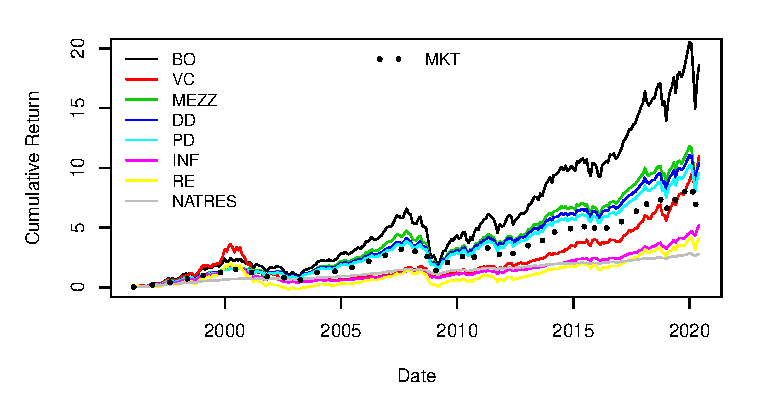
\includegraphics{Figures/Cumulative_Returns.eps}
%	\caption{PREQIN 2020:  Cumulative USD returns implied by the MSCI World factor models from Table 
% \ ref{tab:average_coefs} from 1996-01-31 until 2020-05-31.}
%%\end{figure}


\begin{figure}[H]
	\centering
	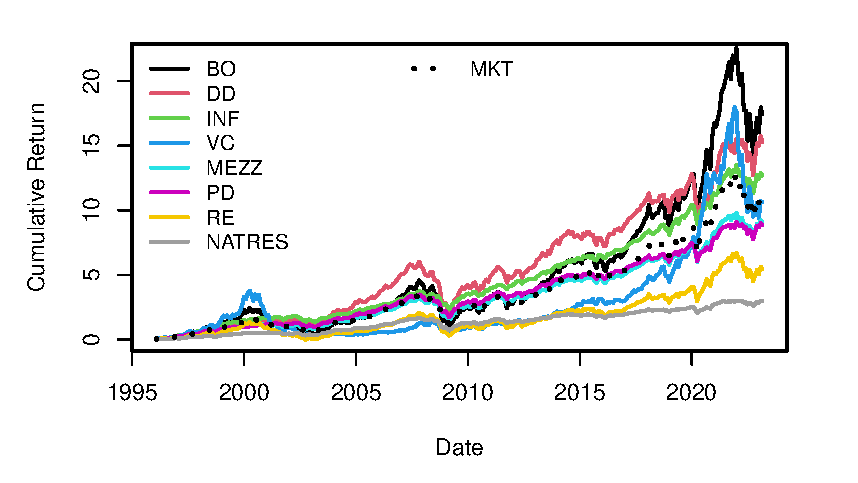
\includegraphics{Figures/Cumulative_Returns_2023_1996.eps}
	\caption{PITCHBOOK 2023: Cumulative USD returns implied by the five-factor models from Table \ref{tab:average_coefs_2023} from 1996-01-31 until 2023-02-28.}
	\label{fig:cum_returns_2023}   
\end{figure}




\subsection{Idiosyncratic returns for Buyout funds}
\label{sec:idiosyncratic_BO}

In this section, we apply the idiosyncratic return estimation method described in subsection \ref{sec:error_term_estimation} for BO funds.
Here we use a starting point an ensemble of the MSCI market factors similar to the one described in Table \ref{tab:average_coefs_2023}.
Now we however only include fund-size-weighted datasets to reduce the long computation time that comes with this brute-force approach\footnote{Estimation for the reduced Buyout ensemble takes around three days on a 2023 MacBook with 12 CPU cores and parallel processing.}.
Specifically, we use an ensemble of 40 two-factor models $4 \times 2 \times 5$  with (i) second factors (HML, SMB, HDY-MKT, QLT-MKT) (ii) quadratic and least absolute deviance loss function $L()$, and (iii) maximum months 120, 150, 180, 210, 240.
The average factor loadings of the five-factor model are fortunately very similar to the ones from Table \ref{tab:average_coefs_2023}:  
MKT-RF (1.46), 
HML (-0.09), 
SMB (-0.10), 
HDY-MKT (-0.15), and 
QLT-MKT (-0.09).

In the second step, we apply componetwise $L_2$ boosting (CLB) with 200 iterations for each two-factor ensemble, a damper factor of 0.33, and return bounds of plus and minus $100\%$.
For each of the 40 ensembles, we start with a vector of 307 zeros for $e$  (i.e. 307 monthly observations from 1998-03-31 until 2022-06-30).
After all CLB algorithms have been terminated, we average over all 40 error term series and public factor models to obtain our final estimate for $e$ and $\beta$.
Since only 46/307=15\% monthly errors are filled with values other than zero in the final $e$ vector, our estimated error term series can be considered relatively sparse.
On a quarterly basis we still have 43/96=45\% non-zero error terms from 1998 until 2022.
Yet two quarters exhibit quite extreme idiosyncratic returns of around +30\% or larger as depicted in Figure \ref{fig:clb_idio}.

\begin{figure}[H]
	\centering
	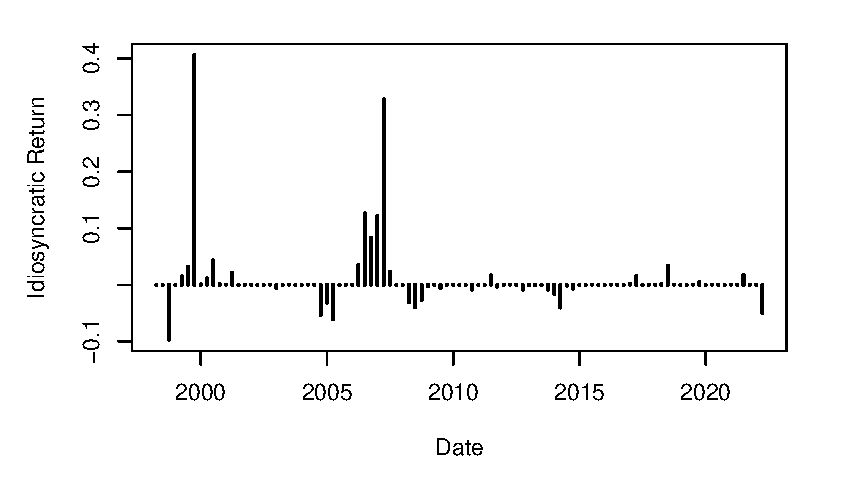
\includegraphics{Figures/msci_market_factors/XErrorSeriesBO}
	\caption{Idiosyncratic returns estimated by componentwise $L_2$ boosting for fund type BO in the period from 1998-03-31 until 2022-03-31.}
	\label{fig:clb_idio}
\end{figure}

For illustration and comparison with other BO return series, we map the monthly returns to quarterly returns in Figures \ref{fig:clb_idio} and \ref{fig:clb_total} and analyze the period from 1998-03-31 until 2022-03-31.
Figure \ref{fig:clb_total} nicely depicts that adding the error term estimates to our public factor model closely aligns the Average 2-Factor Models + Error series to the NAV returns of Cambridge Associates (CA), Preqin and Pitchbook.\footnote{Because of missing data, we fill the first quarters of the Pitchbook series with CA returns (from 1998-03-31 until 1999-09-30) and the first quarters of the Preqin series with CA returns (from 1998-03-31 until 2007-12-31).
}
\textcolor{darkgreen}{As outlined in Table \ref{tab:accuracy_measures},} the Pearson correlation coefficients between our Public Factors + Error series and the CA and Pitchbook series are 79\% and 72\%, respectively.
The quarterly average return is relatively high in all three series with 4.7\% (Public Factors + Error), 3.6\% (CA), and 3.5\% (Pitchbook).
However, the standard deviation is considerably larger in our Public Factors + Error series with 15.4\% compared to 5.7\% and 5.1\% observed for CA and Pitchbook NAV returns, respectively.
For comparison, the MSCI Market [Public Factors] return exhibits a 2.7\% [3.8\%] average quarterly return with a standard deviation of 8.8\% [13.9\%].
Interestingly in Figure \ref{fig:clb_total}, the public factor model returns of the average 2-factor model and the 5-factor model exhibit a very similar return pattern that slightly outperforms the MSCI Market return.
Adding our sparse error term vector $e$ to the factor model generates a new return time series that is closer aligned with both NAV return time series.
However, as can be seen in Figure \ref{fig:autocorrelation}, the observed autocorrelation function values for lags 1 and 2 are considerably smaller in our Average 2-Factor Models + Error series with 12.4\% and 12.0\% than in the CA (35.6\% and 28.7\%), Preqin (44.2\% and 25.2\%) and Pitchbook (41.3\% and 32.7\%) cases.
Our boosting procedure thus can generate return proxies that do not suffer from the smoothing and staleness problems associated with NAV returns.

\begin{figure}[H]
	\centering
	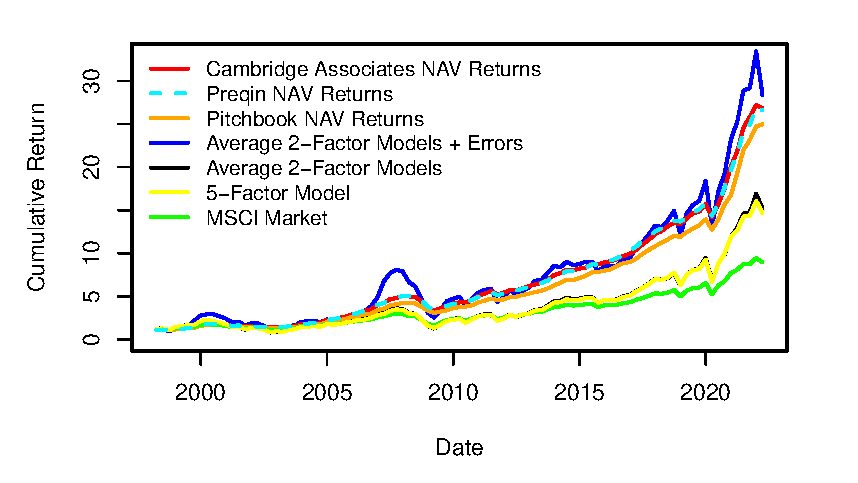
\includegraphics{Figures/msci_market_factors/XTotalErrorSeriesBO}
	\caption{
		Comparison between the total returns for fund type BO implied by our two-factor ensemble and our two-factor ensemble plus the error term from Figure \ref{fig:clb_idio}.
		Both series are contrasted against the NAV Return indices provided by Cambridge Associates, Preqin and Pitchbook and the MSCI stock market index in the period 1998-03-31 until 2022-03-31.
		}
	\label{fig:clb_total}
\end{figure}

\begin{figure}[H]
	\centering
	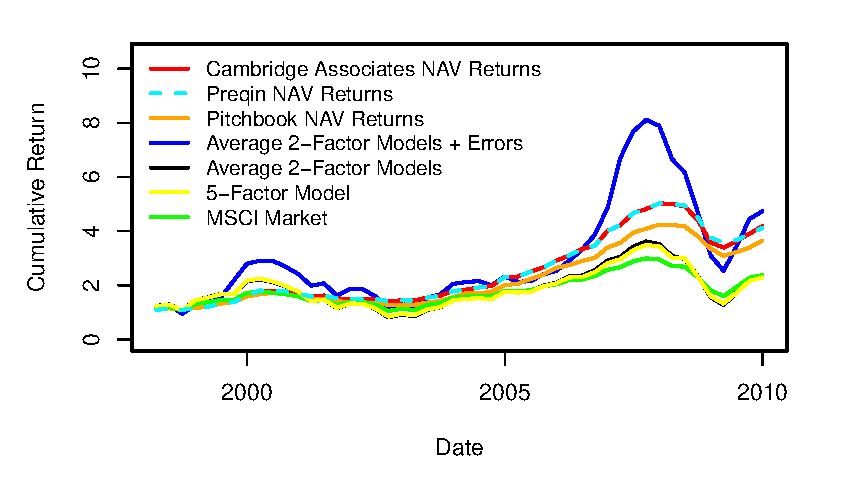
\includegraphics{Figures/msci_market_factors/XTotalErrorSeriesBOpre2010}
	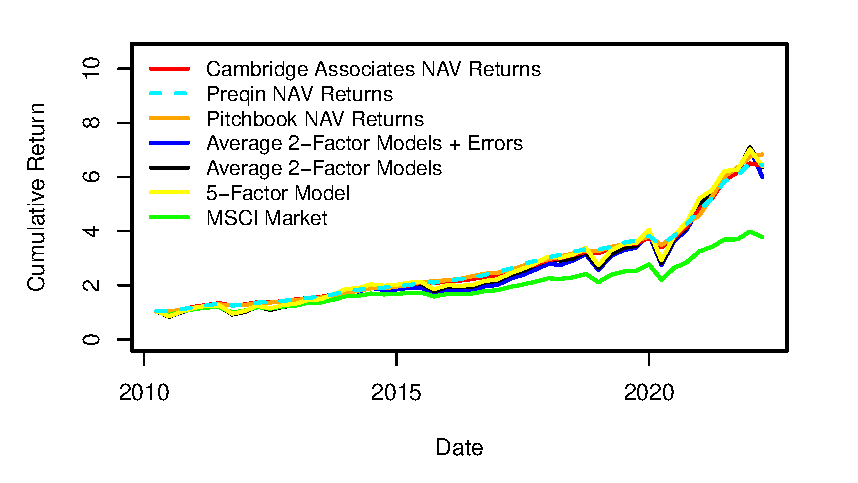
\includegraphics{Figures/msci_market_factors/XTotalErrorSeriesBOpost2010}
	\caption{
		In these two subplots, we split the full time series from Figure \ref{fig:clb_total} into a pre-2010 and post-2010 period.
	}
	\label{fig:clb_pre_post_2010}
\end{figure}

\begin{figure}[H]
	\centering
	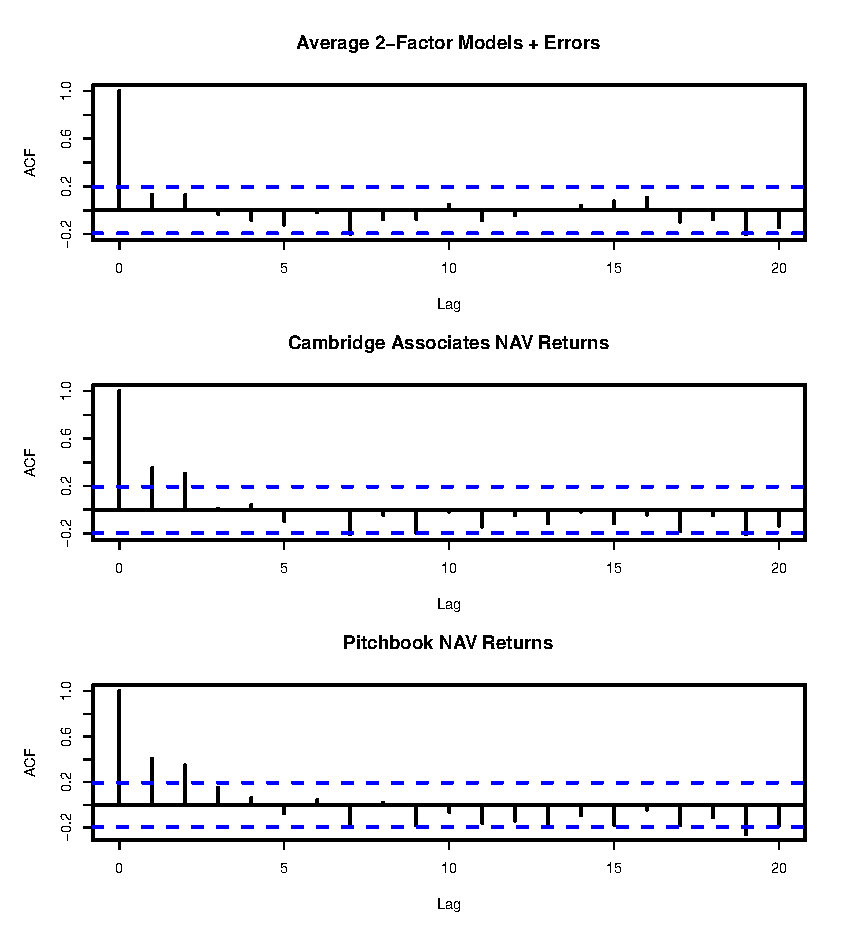
\includegraphics{Figures/ACFunBO}
	\caption{
		Comparison between the autocorrelation functions of our total return time series and the NAV-return time series of Cambridge Associates, Preqin and Pitchbook.
	}
	\label{fig:autocorrelation}
\end{figure}

In Figure \ref{fig:clb_pre_post_2010}, we split Figure \ref{fig:clb_total} in a pre-2010 and a post-2010 period.
We observe a big difference between the Average 2-Factor Models and the Average 2-Factor Models + Errors series in the period before 2010.
However after 2010, all public factor model returns (with and without errors) seem closely aligned with the CA and Pitchbook NAV return indices.
Certainly, this result does not come by surprise as Figure \ref{fig:clb_idio} displays all larger error terms before 2010.
From these analyses it remains unclear if the time-consuming error term estimation is always necessary since the average of the two-factor models alone can adequately price BO cash flows in the more recent past.
% In appendix \ref{sec:vc_errors}, we receive a similar result for VC returns.

Finally, table \ref{tab:error_summary} reports the summary statistics for the error terms to address the question if Buyout (and other fund types) outperformed the public market on a risk-adjusted basis.
The extremely high values for skewness and kurtosis challenge the validity of using the mean of the error term series as measure for the expected outperformance, i.e., $\alpha = E [ e ]$.
Supposedly, the median gives a more realistic approximation for practical purposes since asymptotic behavior cannot be expected for time series of length 100.


% LaTeX table generated in R 4.3.1 by xtable 1.8-4 package
% Fri Sep 20 20:28:23 2024

\begin{table}[ht]
	\centering
	\begin{tabular}{l rrrrrrr}
		{NAV Return} & {MAE} & {MSE} & {RMSE} & {MAPE} & {NMSE} & {rSTD} & {Pearson} \\ 
		\hline
		\hline
		Cambridge A. & 0.085 & 0.013 & 0.115 & 1.918 & 0.561 & 2.448 & 0.785 \\  
	 	PitchBook & 0.092 & 0.015 & 0.122 & 2.298 & 0.636 & 2.605 & 0.723 \\   
	 	Preqin & 0.088 & 0.014 & 0.119 & 1.883 & 0.597 & 2.526 & 0.759 \\ 
		\hline
		\hline
	\end{tabular}
	\caption{
		\textcolor{darkgreen}{
			Quantitative measures of distance between our "2-Factor Models + Error" time series and three NAV-return indices for BO funds as depicted in Figure \ref{fig:clb_total}.
			For the \emph{quarterly} return series, we calculate 
			Mean Absolute Error (MAE),
			Mean Squared Error (MSE),
			Root Mean Squared Error (RMSE),
			Mean Absolute Percentage Error (MAPE),
			Normalized Mean Squared Error (NMSE),
			relative Standard Deviation (rSTD)
			and Pearson correlation.
			}
		}
	\label{tab:accuracy_measures}
\end{table}


\begin{table}[ht]
	\centering
	\begin{tabular}{l | c c c c | c}
		Type & Mean  & Stdv. & Skew. & Kurt.  & Percentage filled \\
		\hline 
		\hline
		BO & 1.12 \% & 6.44 \% & 432 \% & 2081 \% & 44 \% = 45 / 102  \\ 
		VC & 1.33 \% & 12.36 \% &  553 \% & 3827 \% & 62 \% = 61 / 99 \\ 
		RE & 1.06 \% & 16.84 \% & -9 \% & 1799 \% & 51 \% = 50 / 98 \\ 
		INF & 0.91 \% & 11.15 \% & 404 \% & 2579 \% & 36 \% = 34 / 94  \\ 
		NATRES  & 5.77 \% & 41.31 \% & 794 \% & 6887 \% & 36 \% = 36 / 99 \\ 
		PD & 1.05 \% & 5.70 \% & 420 \% & 2166 \% & 44 \% = 34 / 77 \\ 
		\hline 
		\hline 
	\end{tabular} 
	\caption{
		Quarterly error term return summary for various fund segments.
		The percentage filled column gives us the number of quarters with non-zero error terms as determined by the sparse componentwise $L_2$ boosting algorithm; the remaining unfilled quarters show zero idiosyncratic returns.
		Thus, the percentage filled column is a measure of sparseness for our CLB method.
		The median error term is 0 for all reported fund segments due to this sparseness.
	}
\label{tab:error_summary}
\end{table}

\subsection{Model limitations for other fund types}

\textcolor{darkgreen}{
	In this section, we analyze the estimated error-term time series for other private capital fund types, as shown in Appendix \ref{sec:error_terms_other_fund_types}.
	Similar to the BO case, the error-term time series for VC, RE, DD, INF, NATRES, MEZZ, and PD funds are sparse, with most estimated errors being zero. 
	Generally, volatility clusters of several large positive and negative errors only appear infrequently or as single large outliers. 
	However, two irregular and potentially problematic patterns can be identified in the idiosyncratic return time series.
}

\textcolor{darkgreen}{
	First, our error-term estimation methodology sometimes produces unreliable results at the beginning and end of the time series.
	This is especially prominent at the end of the VC error series with a quarterly return of +200\% for the first quarter of 2022 (Figure \ref{fig:clb_idio_VC}). 
	The RE errors start with a return of around -100\% (Figure \ref{fig:clb_idio_RE}).
	The last MEZZ error term is around -50\% (Figure \ref{fig:clb_idio_MEZZ}) and the final PD error term is over +30\% (Figure \ref{fig:clb_idio_PD}).
	Due to the frequent outliers at the beginning and end of the time series, we recommend that researchers always discount or exclude at least the first and last observations of the error-term series generated by our method. 
	For these quarters, it appears more reliable to use only the factor-model returns without including the error terms.
	Alternatively, we could rerun our error-term estimation method on a trimmed cash flow dataset if outliers are found at the beginning or end, though this approach is more computationally intensive.
}

\textcolor{darkgreen}{
	Second, for asset classes with relatively few funds in our dataset, the error-term time series can display quarters with extreme idiosyncratic return estimates, particularly around the 2007-08 financial crisis.
	Between 2007 and 2009, we observe an almost +80\% return for DD funds (Figure \ref{fig:clb_idio_DD}) and an almost +400\% return for NATRES funds (Figure \ref{fig:clb_idio_NATRES}).
	INF funds also exhibit two negative returns of around -20\% and two positive returns larger than +50\% in the period between 2005 and 2008 (Figure \ref{fig:clb_idio_INF}).
	However, in some instances, the increased volatility of error terms during the 2007-08 financial crisis may realistically represent actual market conditions. 
	In other cases, such as a 400\% return in a single quarter, it is clearly reasonable to introduce a return cap, limiting error estimates to no more than, e.g., 100\% per quarter.
}

\textcolor{darkgreen}{
	Despite the two issues mentioned above, the cumulative return time series for many of the fund types discussed show patterns similar to their NAV-return benchmarks. 
	Only the cumulative returns for NATRES and MEZZ appear noticeably different when examined visually.
≠
}


\iffalse

\subsection{Integrated public and private risk management}
\label{sec:integrated_risk}

In typical applications, we want to use our SDF models to analyze a blended portfolio of different private capital funds rather than investigate the factor exposure of a specific fund type.
In this case, we favor the bottom-up aggregation of SDF models to avoid overfitting.
Here, it is also straightforward to match the regional factor indices fund by fund.
In contrast, top-down selection of the 'best' SDF model for portfolio-level cash flows is likely to overfit with strongly varying SDF models for a given portfolio over time.

We consider two sets of ensembles when determining the factor exposure of actual PE portfolios.
The balanced ensemble is the set of all valid models for a given fund type, i.e., exactly the set $M^*$ as defined in subsection \ref{sec:model_averaging}.
The best ensemble is the size-$M^{**}$ subset of the balanced ensemble containing SDFs that best describes a given fund's cash flows in terms of absolute net present value error. 
Consequently, the number of components in the best ensemble is smaller than in the balanced ensemble $M^{**} \leq M^*$.
The comparison of the best and balanced model coefficients assesses how much the benchmarked portfolio's investment style differs from the average factor exposure of similar private capital portfolios.

For a sample portfolio of 100 funds visualized in figure \ref{fig:coef_barchart_100_pofo}, we see that the balanced model exhibits a MKT-RF coefficient slightly larger than one but the best SDF model MKF-RF coefficient is closer to 1.2.
This result implies higher than average market exposure for our portfolio.
Similarly, the best factor coefficients for HDY-MKT, QLT-MKT, and SMB are also higher than for the balanced ensemble.
Only the HML factor coefficient is basically the same for the best and balanced model.

Assume the asset owner of this PE portfolio is also invested in public markets.
For an integrated risk management application, the factor model derived by the best ensemble can be used as a public factor representation of the PE portfolio.
Established factor representations of any (public or private) portfolio shall be easily compatible with the asset owner's risk management framework.
Relevant methods to calculate risk measures like volatility, value-at-risk, or expected shortfall for public factor models shall be readily available in any investment risk department. 
This general approach works best if (i) the PE portfolio is diversified, and (ii) the public portfolio is still considerably larger than the PE allocation.
These conditions render an SDF model tracking error that is small in (i) absolute and (ii) relative terms and can thus be neglected.

\begin{figure}[H]
	\centering
	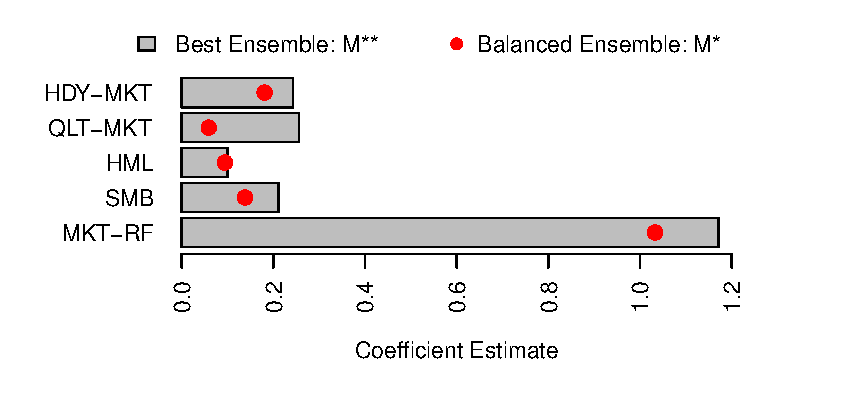
\includegraphics{Figures/Coefs100Pofo}
	\caption{Coefficient estimates of best and balanced linear SDF model for a sample portfolio consisting of 100 private capital funds.}
	\label{fig:coef_barchart_100_pofo}
\end{figure}

\fi


\section{Conclusion}
\label{sec:conclusion}

In summary, this paper introduces a straightforward ensemble method designed to translate private equity cash flows into a public factor model and an error term time series. 
The versatility of this method is evident in its applicability, serving two primary purposes: 
(i) exploring the public market factor exposures of various private equity fund types or strategies and (ii) analyzing specific private equity portfolios. 
By enabling the use of factor loadings and error terms in integrated risk management, this approach establishes a standardized foundation for comparing the risk exposure of public and private asset portfolios.

This innovative analysis represents a valuable addition to traditional methods for characterizing the style and risk of private equity investments, providing investors with additional insights. 
Our error term analysis, particularly for Buyout funds, reveals a temporal shift in the significance of the error term in describing total returns. 
Before 2010, the error term played a crucial role, whereas after 2010, the public factor model alone proved sufficient to price Buyout cash flows. 
Moreover, our error term estimates exhibit too extreme higher moments to be adequately  described by lower order summary statistics like the mean value alone.
This, in turn, casts doubts on the usefulness of the exptected outperformance term $\alpha = E [ e ]$ in the context of private capital returns.
Notably, our empirical application yields total return time series for private equity segments with significantly lower autocorrelations than traditional NAV-return time series.
\textcolor{darkgreen}{
However, our error-term estimation methodology sometimes produces unreliable outliers, particularly at the beginning and end of the time series, which researchers should consider trimming.
}

Looking forward, there are promising avenues for refining our approach. 
Firstly, enhancing the (i) simple ensemble approach for the public factor model and (ii) brute-force componentwise $L_2$ boosting for the error term can be achieved through more efficient machine learning algorithms \citep{B12}.
Additionally, integrating cross-validation techniques can enhance the reliability of identifying valid SDF models compared to our current quantile-based procedure, as briefly mentioned in this article.
Finally, to validate the robustness of our findings, further studies should replicate our results using alternative private and public data sources beyond Pitchbook and MSCI data. 
These potential enhancements and validations are essential steps toward strengthening the credibility and generalizability of our proposed methodology.

%% References
\bibliographystyle{apalike}
\bibliography{ref}

% Appendix
\appendix

\clearpage


\section{Comparison to competing approaches}
\label{sec:comparison}

\textcolor{darkgreen}{
	In this appendix, we compare our two-step methodology to potentially simpler competitor models highlighting advantages as well as disadvantages associated with each model.
	In this context, it is paramount to explain which general intricacies arise when researchers want to estimate a regression model $R = \beta X + e$ with private equity returns $R$ as dependent variable and a linear factor model $\beta X$ plus error term $e$ on the right-hand side.
}

\textcolor{darkgreen}{
	The first fundamental challenge is accurately measuring private equity returns $R$, as fund NAVs are impacted by intermediate cash flows and stale pricing, both of which are difficult to avoid for closed-end funds operating in illiquid markets. 
	The second challenge is estimating a factor model $\beta X$ when only incomplete return time series or cash flow data are available.
	The third problem is to derive the error term $e$ that comes with a factor model $\beta X$ given the same fundamental problems.
}

\subsection{Return measurement}
% Horizon IRR and NAV returns

\textcolor{darkgreen}{
	The most straightforward alternative to our model would be a "precise" measurement of "true" PE fund returns.
	Given well-behaved PE return time-series, factor model estimation and error term calculation can be simply done by a linear Ordinary Least Squares (OLS) regression.
	However, in practice true PE returns can be only approximated by so-called Horizon Internal Rate of Returns (Horizon IRRs) or NAV returns (or variants thereof).
}

\textcolor{darkgreen}{
	Horizon IRR is a measure used to evaluate the performance of private equity investments over a specific time period, accounting for both interim cash flows and changes in NAV.
	Unlike traditional IRR, which focuses on the full lifetime cash flows of an investment, Horizon IRR assesses returns within a given investment horizon, typically over shorter periods like one or several years. 
	This metric is often used for benchmarking and performance comparison across funds during specific periods.
	\[
	\mathrm{IRR}_{t_1,t_2}^{horizon} := \arg \min_{r \in \mathbb{R}} 
	\left| 
	{NAV}_{t_1} -
	\sum_{t=t_1}^{t_2} \frac{{CF}_t}{(1 + r)^{t-t_1}} 
	- \frac{{NAV}_{t_2}}{(1 + r)^{t_2-t_1}}
	\right|
	\stackrel{!}{=} 0
	\]
}

\textcolor{darkgreen}{
	The connection between Horizon IRR and NAV returns lies in their shared focus on interim valuations. 
	NAV returns capture the percentage change in a private equity fund's NAV, adjusted for distributions and contributions, and are often calculated on a quarterly or annual basis. 
	\[
	R_{t_1, t_2}^{\mathrm{NAV}} := \frac{{NAV}_{t_2} - \sum_{t=t_1}^{t_2} {CF}_t }{{NAV}_{t_1}}
	\]
	Horizon IRR incorporates NAV returns by considering both the periodic changes in NAV and cash flows (capital calls and distributions) during the investment horizon, providing a more time-weighted performance measure that accounts for both realized and unrealized gains. 
	Unfortunately, the inherent stale pricing of PE funds' NAVs yields autocorrelated NAV returns as previously exemplified by Figure \ref{fig:autocorrelation}.
	Thus, NAV returns and Horizon IRRs can only be considered as proxy returns.
	}
	
\subsection{Factor-model estimation}
% \cite{dimson1979risk} regression

\textcolor{darkgreen}{
	The \cite{dimson1979risk} beta approach -- initially developed for public shares that are subject to infrequent trading -- is particularly useful for estimating factor loadings in private equity returns, where stale pricing (of NAV appraisals) can lead to asynchronous movements with market factors. 
	Traditional beta estimation assumes contemporaneous correlation between asset returns and factor returns, which may not hold for illiquid, non-traded assets like private equity. 
	The \cite{dimson1979risk} beta corrects for this by incorporating lagged factor returns in the OLS regression, capturing delayed or smoothed responses to market-wide movements. 
	This method potentially improves the accuracy of factor loading estimates, reflecting a more realistic sensitivity of private equity returns to systematic risk factors.
	As dependent variable for a \cite{dimson1979risk} regression, we could use NAV returns or Horizon IRRs.
	\[
	R_t^{\mathrm{Dimson}} := 
	\alpha + \sum_{l=0}^L \sum_j \beta_{j,l} F_{j,t-l} + e_{t}
	\]
	Unfortunately, this method is not helpful to determine the "true" total PE return as the error terms in the formula above are directly derived from the stale returns that serve as dependent variable in the regression. 
}

\textcolor{darkgreen}{
	\cite{DLP12}, \cite{KN16}, \cite{ACGP18} propose factor-models estimators that use cash flows instead for return time series to completely avoid the (fundamental) stale pricing problem associated with NAVs.
	Our method is based on the \cite{DLP12} approach.
}

\subsection{Error-term derivation}
% \cite{ACGP18} MCMC

\textcolor{darkgreen}{
	The advanced \cite{ACGP18} ansatz aims at creating a Markov Chain Monte Carlo (MCMC) sampler which equilibrium distribution matches the distribution of latent private equity returns denoted by $g_t$.
	While estimating the MCMC they further decompose the PE returns by a linear multi-factor model $g_t = \alpha + \beta^{'} F_t + f_t + r_t^{rf}$ where $ r_t^{rf}$ denotes the risk-free rate and $f_t$ is perceived as asset-class specific latent factor (i.e., the error term) with mean zero that is orthogonal to the traded factors, $F_t$.
	The corresponding factor loadings $\beta$ need to be subsequently updated in each MCMC iteration after a new candidate for $g_t$ has been drawn via "a standard regression draw" \cite[internet appendix, p.4]{ACGP18}.
	In the final step, each MCMC iteration samples a nuisance parameter, assumed to follow a normal distribution. 
}

\textcolor{darkgreen}{
	In summary, their approach first samples total PE returns by normal draws around the factor-model mean for each date and then -- as a second step -- updates the public factor model via a multi-variate Least Absolute Deviations (LAD) regression on this total return series.
	In contrast, we first combine multiple, potentially simpler (uni- or bi-variate) factor models by model averaging and then -- in the second step -- directly estimate the time-series of idiosyncratic returns via a straightforward but brute-force algorithm.
	A minor drawback of the \cite{ACGP18} framework is its inherent complexity, which, along with its Bayesian nature, offers researchers considerable flexibility in selecting priors and making subtle design decisions.
	In other words, several variations of the \cite{ACGP18} algorithm appear reasonable and worth investigating.
}
% \clearpage


\section{Pitchbook}
\label{sec:pitchbook}




\newcommand{\scaleWidth}{14cm}

% latex table generated in R 4.2.1 by xtable 1.8-4 package
% Thu May 11 10:54:20 2023
\begin{table}[ht]
	\centering
	\resizebox{\scaleWidth}{!}{% use resizebox with textwidth
		\begin{tabular}{lllllll}
			Type & MKT-RF & HML & SMB & HDY-MKT & QLT-MKT & Alpha \\ 
			\hline
			\hline
			%ALL & 1.23 (0.24) & -0.13 (0.06) & -0.18 (0.07) & -0.26 (0.13) & 0.04 (0.1) & -0.007 (0.02) \\ 
			BO & 1.33 (0.27) & -0.09 (0.04) & -0.14 (0.05) & -0.18 (0.09) & -0.11 (0.07) & 0.007 (0.017) \\ 
			DD & 0.83 (0.28) & 0.27 (0.06) & 0.35 (0.04) & 0.51 (0.08) & -0.4 (0.07) & 0.031 (0.043) \\ 
			%FOF & 0.56 (1.77) & -0.04 (0.25) & -0.51 (0.39) & -0.28 (0.79) & -0.27 (1.27) & 0.126 (0.245) \\ 
			INF & -0.29 (0.75) & -0.06 (0.11) & -0.31 (0.35) & -0.33 (0.43) & 0.46 (0.67) & 0.104 (0.1) \\ 
			MEZZ & 0.58 (0.17) & 0.03 (0.04) & 0.13 (0.05) & 0.06 (0.06) & -0.09 (0.09) & 0.024 (0.017) \\ 
			NATRES & 0.7 (0.35) & 0.06 (0.12) & 0.17 (0.18) & 0.17 (0.18) & -0.4 (0.33) & -0.019 (0.067) \\ 
			PD & 0.19 (0.43) & 0.15 (0.04) & 0.17 (0.05) & 0.24 (0.18) & -0.22 (0.23) & 0.068 (0.051) \\ 
			%PE & 1.32 (0.28) & -0.16 (0.08) & -0.19 (0.1) & -0.28 (0.17) & 0.11 (0.1) & -0.005 (0.023) \\ 
			RE & 2.02 (0.37) & 0.1 (0.08) & -0.07 (0.15) & 0.04 (0.19) & -0.55 (0.16) & -0.063 (0.047) \\ 
			%SEC & 1.63 (0.46) & -0.16 (0.05) & -0.15 (0.11) & -0.22 (0.16) & 0.32 (0.25) & -0.031 (0.036) \\ 
			VC & 1.41 (0.66) & -0.53 (0.08) & -0.7 (0.04) & -0.97 (0.18) & 0.63 (0.1) & -0.03 (0.071) \\ 
			\hline
			MKT & 1 & 0 & 0 & 0 & 0 & 0 \\ 
			\hline
			\hline
		\end{tabular}
	}
	\caption{
		PITCHBOOK 2023 ALPHA: Multivariate five-factor models obtained by simple coefficient averaging (with standard deviations in parenthesis).
		The ``Alpha'' term gives the average monthly outperformance.
	} 
	\label{tab:average_coefs_2023_alpha}
\end{table}


% latex table generated in R 4.2.1 by xtable 1.8-4 package
% Wed Jun 28 10:08:33 2023
\begin{table}[ht]
	\centering
	\begin{tabular}{llllll}
		Type & MKT & TERM & CORP & HY & LIQ \\ 
		\hline
		\hline
		ALL & 1.49 (0.14) & -0.25 (0.09) & -1.08 (0.34) & -0.62 (0.22) & -0.18 (0.05) \\ 
		BO & 1.56 (0.11) & -0.15 (0.01) & -0.75 (0.1) & -0.4 (0.02) & -0.01 (0.07) \\ 
		DD & 0.52 (0.12) & 0.34 (0.07) & 1.39 (0.17) & 0.73 (0.15) & 0.37 (0.06) \\ 
		FOF & 1.45 (0.21) & -0.3 (0.08) & -1.34 (0.22) & -0.9 (0.34) & -0.37 (0.17) \\ 
		INF & 0.59 (0.15) & 0.21 (0.07) & 0.62 (0.32) & 0.63 (0.16) & 0.24 (0.09) \\ 
		MEZZ & 0.6 (0.1) & 0.25 (0.08) & 0.78 (0.39) & 0.41 (0.17) & 0.23 (0.06) \\ 
		NATRES & 0.37 (0.11) & -0.23 (0.19) & 0.16 (0.42) & -0.42 (0.44) & 0.17 (0.18) \\ 
		PD & 0.4 (0.24) & 0.39 (0.23) & 1.24 (0.29) & 0.81 (0.34) & 0.23 (0.12) \\ 
		PE & 1.62 (0.13) & -0.23 (0.1) & -0.99 (0.37) & -0.58 (0.25) & -0.17 (0.09) \\ 
		RE & 1.47 (0.33) & -0.58 (0.17) & -3.44 (0.23) & -1.93 (0.41) & -0.49 (0.1) \\ 
		SEC & 1.71 (0.19) & -0.23 (0.1) & -0.97 (0.61) & -0.87 (0.44) & -0.25 (0.15) \\ 
		VC & 2.4 (0.42) & -0.75 (0.11) & -3.77 (0.79) & -2.21 (0.36) & -0.57 (0.05) \\ 
		\hline
		MKT & 1 & 0 & 0 & 0 & 0 \\ 
		\hline
		\hline
	\end{tabular}
	\caption{PITCHBOOK IBOXX MIX 2023: 
		Average coefficients of iBoxx factor models with standard deviation in parentheses.} 
	\label{tab:average_coefs_iboxx}
\end{table}


\iffalse

% latex table generated in R 4.2.1 by xtable 1.8-4 package
% Wed Jun 28 10:44:39 2023
\begin{table}[ht]
	\centering
	\begin{tabular}{rrrrrr}
		& Mean & Stdv & Mean.ex & Stdv.ex & Sharpe \\ 
		\hline
		\hline
		ALL & 0.107 & 0.239 & 0.091 & 0.219 & 0.414 \\ 
		BO & 0.123 & 0.256 & 0.107 & 0.236 & 0.453 \\ 
		DD & 0.083 & 0.131 & 0.067 & 0.109 & 0.613 \\ 
		FOF & 0.094 & 0.229 & 0.078 & 0.209 & 0.372 \\ 
		INF & 0.076 & 0.129 & 0.060 & 0.107 & 0.565 \\ 
		MEZZ & 0.078 & 0.132 & 0.062 & 0.110 & 0.568 \\ 
		NATRES & 0.041 & 0.082 & 0.026 & 0.057 & 0.452 \\ 
		PD & 0.070 & 0.111 & 0.054 & 0.088 & 0.614 \\ 
		PE & 0.119 & 0.260 & 0.102 & 0.241 & 0.425 \\ 
		RE & 0.070 & 0.218 & 0.054 & 0.199 & 0.271 \\ 
		SEC & 0.122 & 0.273 & 0.106 & 0.254 & 0.418 \\ 
		VC & 0.133 & 0.354 & 0.116 & 0.336 & 0.345 \\ 
		\hline
		MKT & 0.089 & 0.177 & 0.073 & 0.156 & 0.469 \\ 
		\hline
		\hline
	\end{tabular}
	\caption{
		PITCHBOOK IBOXX MIX 2023:
		Annualized returns of iBoxx five-factor models.
		The underlying monthly returns are based on iBoxx bond indices (for TERM, CORP, HY, LIQ) and the MSCI World for the MKT factor (in USD) from 1999-01-31 to 2023-02-28.
	} 
	\label{tab:ann_returns_iboxx}
\end{table}
\fi

\clearpage


\begin{figure}[H]
	\centering
	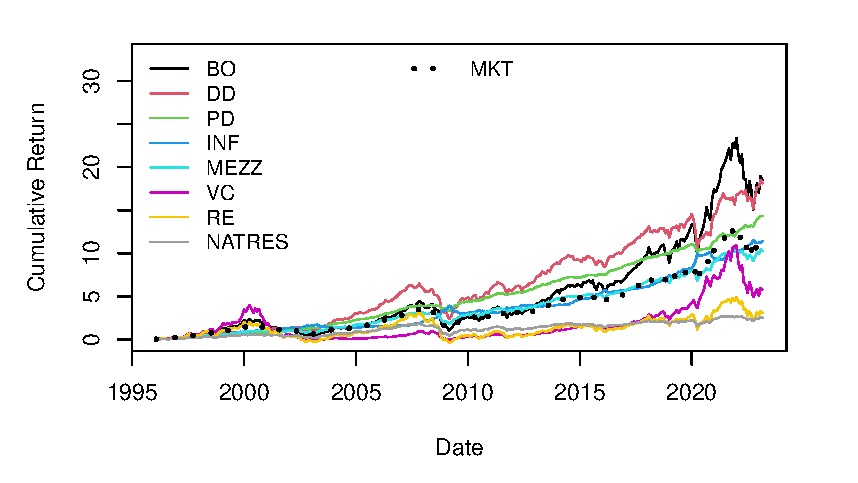
\includegraphics{Figures/Cumulative_Returns_2023_Alpha.eps}
	\caption{PITCHBOOK 2023 ALPHA: Cumulative USD returns implied by the MSCI World factor models from Table \ref{tab:average_coefs_2023} from 1999-01-31 until 2023-02-28.}
	\label{fig:cum_returns_2023_alpha}   
\end{figure}


\begin{figure}[H]
	\centering
	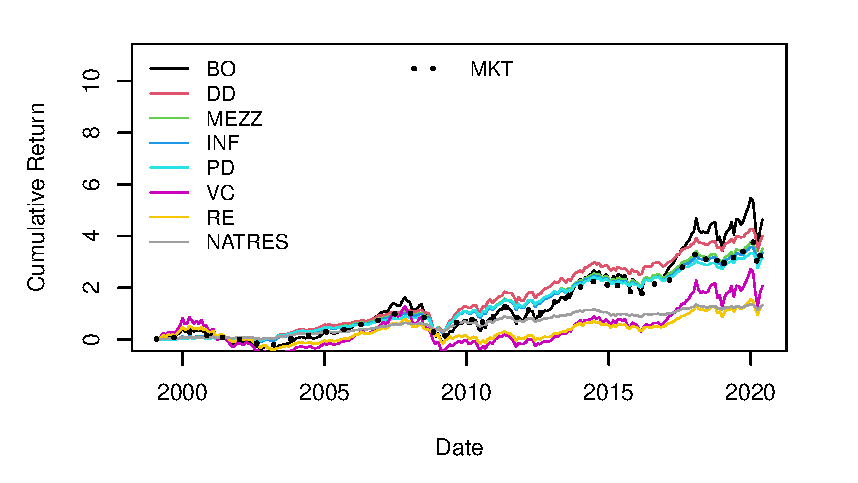
\includegraphics{Figures/Cumulative_Returns_2023_Bond.eps}
	\caption{PITCHBOOK 2023 BOND: Cumulative USD returns implied by the MSCI World factor models from Table \ref{tab:average_coefs_2023} from 1999-01-31 until 2023-02-28.}
	\label{fig:cum_returns_2023_iboxxx}
\end{figure}

\clearpage


\newcommand{\segment}{BO}

\section{Idiosyncratic returns for VC funds}
\label{sec:vc_errors}


% Factor Model Returns + Errors for VC
\renewcommand{\segment}{VC}

\begin{figure}[H]
	\centering
	\includegraphics{Figures/msci_market_factors/XErrorSeries\segment}
	\caption{
		Idiosyncratic returns estimated by componentwise $L_2$ boosting for fund type \segment \ in the period from 1998-03-31 until 2022-03-31.
		For the last quarter (2022-03-31), we see an extreme return outlier of more than 200\%.
	}
	\label{fig:clb_idio_\segment}
\end{figure}

\begin{figure}[H]
	\centering
	\includegraphics{Figures/msci_market_factors/XTotalErrorSeries\segment}
	\caption{
		Comparison between the total returns for fund type \segment \ implied by our two-factor ensemble and our two-factor ensemble plus the error term from Figure \ref{fig:clb_idio}.
		Both series are contrasted against the NAV Return indices provided by Cambridge Associates and Pitchbook and the MSCI stock market index in the period 1998-03-31 until 2022-03-31.
	}
	\label{fig:clb_total_\segment}
\end{figure}

\begin{figure}[H]
	\centering
	\includegraphics{Figures/msci_market_factors/XTotalErrorSeries\segment pre2010}
	\includegraphics{Figures/msci_market_factors/XTotalErrorSeries\segment post2010}
	\caption{
		In these two subplots, we split the full \segment \ time series from Figure \ref{fig:clb_total_\segment} into a pre-2010 and post-2010 period.
		Similar to the BO case in Figure \ref{fig:clb_pre_post_2010}, we see diverse return time series pre 2010 but after 2010 all three public factor model returns (with and without error terms) closely match the two NAV return series.
	}
	\label{fig:clb_pre_post_2010_\segment}
\end{figure}


% Factor Model Returns + Errors for RE
\renewcommand{\segment}{RE}

\section{Idiosyncratic returns for \segment \ funds}
\label{sec:errors_\segment}

\begin{figure}[H]
	\centering
	\includegraphics{Figures/msci_market_factors/XErrorSeries\segment}
	\caption{Idiosyncratic returns estimated by componentwise $L_2$ boosting for fund type \segment \ in the period from 1998-03-31 until 2022-03-31.}
	\label{fig:clb_idio_\segment}
\end{figure}

\begin{figure}[H]
	\centering
	\includegraphics{Figures/msci_market_factors/XTotalErrorSeries\segment}
	\caption{
		Comparison between the total returns for fund type \segment \ implied by our two-factor ensemble and our two-factor ensemble plus the error term from Figure \ref{fig:clb_idio_\segment}.
		Both series are contrasted against the NAV Return indices provided by Cambridge Associates and Pitchbook and the MSCI stock market index in the period 1998-03-31 until 2022-03-31.
	}
	\label{fig:clb_total_\segment}
\end{figure}

\begin{figure}[H]
	\centering
	\includegraphics{Figures/msci_market_factors/XTotalErrorSeries\segment pre2010}
	\includegraphics{Figures/msci_market_factors/XTotalErrorSeries\segment post2010}
	\caption{
		In these two subplots, we split the full \segment \ time series from Figure \ref{fig:clb_total_\segment} into a pre-2010 and post-2010 period.
	}
	\label{fig:clb_pre_post_2010_\segment}
\end{figure}


% Factor Model Returns + Errors for DD
\renewcommand{\segment}{DD}

\section{Idiosyncratic returns for \segment \ funds}
\label{sec:errors_\segment}

\begin{figure}[H]
	\centering
	\includegraphics{Figures/msci_market_factors/XErrorSeries\segment}
	\caption{Idiosyncratic returns estimated by componentwise $L_2$ boosting for fund type \segment \ in the period from 1998-03-31 until 2022-03-31.}
	\label{fig:clb_idio_\segment}
\end{figure}

\begin{figure}[H]
	\centering
	\includegraphics{Figures/msci_market_factors/XTotalErrorSeries\segment}
	\caption{
		Comparison between the total returns for fund type \segment \ implied by our two-factor ensemble and our two-factor ensemble plus the error term from Figure \ref{fig:clb_idio_\segment}.
		Both series are contrasted against the NAV Return indices provided by Cambridge Associates and Pitchbook and the MSCI stock market index in the period 1998-03-31 until 2022-03-31.
	}
	\label{fig:clb_total_\segment}
\end{figure}

\begin{figure}[H]
	\centering
	\includegraphics{Figures/msci_market_factors/XTotalErrorSeries\segment pre2010}
	\includegraphics{Figures/msci_market_factors/XTotalErrorSeries\segment post2010}
	\caption{
		In these two subplots, we split the full \segment \ time series from Figure \ref{fig:clb_total_\segment} into a pre-2010 and post-2010 period.
	}
	\label{fig:clb_pre_post_2010_\segment}
\end{figure}


% Factor Model Returns + Errors for INF
\renewcommand{\segment}{INF}

\section{Idiosyncratic returns for \segment \ funds}
\label{sec:errors_\segment}

\begin{figure}[H]
	\centering
	\includegraphics{Figures/msci_market_factors/XErrorSeries\segment}
	\caption{Idiosyncratic returns estimated by componentwise $L_2$ boosting for fund type \segment \ in the period from 1998-03-31 until 2022-03-31.}
	\label{fig:clb_idio_\segment}
\end{figure}

\begin{figure}[H]
	\centering
	\includegraphics{Figures/msci_market_factors/XTotalErrorSeries\segment}
	\caption{
		Comparison between the total returns for fund type \segment \ implied by our two-factor ensemble and our two-factor ensemble plus the error term from Figure \ref{fig:clb_idio_\segment}.
		Both series are contrasted against the NAV Return indices provided by Cambridge Associates and Pitchbook and the MSCI stock market index in the period 1998-03-31 until 2022-03-31.
	}
	\label{fig:clb_total_\segment}
\end{figure}

\begin{figure}[H]
	\centering
	\includegraphics{Figures/msci_market_factors/XTotalErrorSeries\segment pre2010}
	\includegraphics{Figures/msci_market_factors/XTotalErrorSeries\segment post2010}
	\caption{
		In these two subplots, we split the full \segment \ time series from Figure \ref{fig:clb_total_\segment} into a pre-2010 and post-2010 period.
	}
	\label{fig:clb_pre_post_2010_\segment}
\end{figure}


% Factor Model Returns + Errors for NATRES
\renewcommand{\segment}{NATRES}

\section{Idiosyncratic returns for \segment \ funds}
\label{sec:errors_\segment}

\begin{figure}[H]
	\centering
	\includegraphics{Figures/msci_market_factors/XErrorSeries\segment}
	\caption{Idiosyncratic returns estimated by componentwise $L_2$ boosting for fund type \segment \ in the period from 1998-03-31 until 2022-03-31.}
	\label{fig:clb_idio_\segment}
\end{figure}

\begin{figure}[H]
	\centering
	\includegraphics{Figures/msci_market_factors/XTotalErrorSeries\segment}
	\caption{
		Comparison between the total returns for fund type \segment \ implied by our two-factor ensemble and our two-factor ensemble plus the error term from Figure \ref{fig:clb_idio_\segment}.
		Both series are contrasted against the NAV Return indices provided by Cambridge Associates and Pitchbook and the MSCI stock market index in the period 1998-03-31 until 2022-03-31.
	}
	\label{fig:clb_total_\segment}
\end{figure}

\begin{figure}[H]
	\centering
	\includegraphics{Figures/msci_market_factors/XTotalErrorSeries\segment pre2010}
	\includegraphics{Figures/msci_market_factors/XTotalErrorSeries\segment post2010}
	\caption{
		In these two subplots, we split the full \segment \ time series from Figure \ref{fig:clb_total_\segment} into a pre-2010 and post-2010 period.
	}
	\label{fig:clb_pre_post_2010_\segment}
\end{figure}


% Factor Model Returns + Errors for MEZZ
\renewcommand{\segment}{MEZZ}

\section{Idiosyncratic returns for \segment \ funds}
\label{sec:errors_\segment}

\begin{figure}[H]
	\centering
	\includegraphics{Figures/msci_market_factors/XErrorSeries\segment}
	\caption{Idiosyncratic returns estimated by componentwise $L_2$ boosting for fund type \segment \ in the period from 1998-03-31 until 2022-03-31.}
	\label{fig:clb_idio_\segment}
\end{figure}

\begin{figure}[H]
	\centering
	\includegraphics{Figures/msci_market_factors/XTotalErrorSeries\segment}
	\caption{
		Comparison between the total returns for fund type \segment \ implied by our two-factor ensemble and our two-factor ensemble plus the error term from Figure \ref{fig:clb_idio_\segment}.
		Both series are contrasted against the NAV Return indices provided by Cambridge Associates and Pitchbook and the MSCI stock market index in the period 1998-03-31 until 2022-03-31.
	}
	\label{fig:clb_total_\segment}
\end{figure}

\begin{figure}[H]
	\centering
	\includegraphics{Figures/msci_market_factors/XTotalErrorSeries\segment pre2010}
	\includegraphics{Figures/msci_market_factors/XTotalErrorSeries\segment post2010}
	\caption{
		In these two subplots, we split the full \segment \ time series from Figure \ref{fig:clb_total_\segment} into a pre-2010 and post-2010 period.
	}
	\label{fig:clb_pre_post_2010_\segment}
\end{figure}


% Factor Model Returns + Errors for PD
\renewcommand{\segment}{PD}

\section{Idiosyncratic returns for \segment \ funds}
\label{sec:errors_pd}

\begin{figure}[H]
	\centering
	\includegraphics{Figures/msci_market_factors/XErrorSeries\segment}
	\caption{Idiosyncratic returns estimated by componentwise $L_2$ boosting for fund type \segment \ in the period from 1998-03-31 until 2022-03-31.}
	\label{fig:clb_idio_\segment}
\end{figure}

\begin{figure}[H]
	\centering
	\includegraphics{Figures/msci_market_factors/XTotalErrorSeries\segment}
	\caption{
		Comparison between the total returns for fund type \segment \ implied by our two-factor ensemble and our two-factor ensemble plus the error term from Figure \ref{fig:clb_idio_\segment}.
		Both series are contrasted against the NAV Return indices provided by Cambridge Associates and Pitchbook and the MSCI stock market index in the period 1998-03-31 until 2022-03-31.
	}
	\label{fig:clb_total_\segment}
\end{figure}

\begin{figure}[H]
	\centering
	\includegraphics{Figures/msci_market_factors/XTotalErrorSeries\segment pre2010}
	\includegraphics{Figures/msci_market_factors/XTotalErrorSeries\segment post2010}
	\caption{
		In these two subplots, we split the full \segment \ time series from Figure \ref{fig:clb_total_\segment} into a pre-2010 and post-2010 period.
	}
	\label{fig:clb_pre_post_2010_\segment}
\end{figure}


% 
\clearpage


\section{Preqin}
\label{sec:preqin}


% latex table generated in R 3.4.2 by xtable 1.8-4 package
% Wed Jul  1 13:54:55 2020
\begin{table}[ht]
	\centering
	\begin{tabular}{l@{\hskip 0.3in}l@{\hskip 0.2in}l@{\hskip 0.2in}l@{\hskip 0.2in}l@{\hskip 0.2in}l@{\hskip 0.1in}}
		Type & MKT-RF & HML & SMB & HDY-MKT & QLT-MKT \\ 
		\hline
		\hline
		BO & 1.33 (0.15) & -0.15 (0.12) & 0.2 (0.03) & 0.3 (0.1) & 0.21 (0.05) \\ 
		DD & 0.96 (0.09) & -0.11 (0.04) & 0.21 (0.01) & 0.14 (0.1) & 0.16 (0.05) \\ 
		%FOF & 1.22 (0.23) & -0.43 (0.09) & -0.24 (0.05) & -0.54 (0.09) & -0.01 (0.04) \\ 
		INF & 0.71 (0.22) & -0.37 (0.06) & -0.33 (0.13) & -0.47 (0.35) & 0.36 (0.11) \\ 
		MEZZ & 1.08 (0.13) & 0.06 (0.1) & 0.14 (0.04) & 0.16 (0.1) & 0.06 (0.11) \\ 
		NATRES & 0.36 (0.27) & -0.04 (0.22) & -0.02 (0.22) & 0.16 (0.36) & 0.11 (0.17) \\ 
		PD & 0.96 (0.08) & -0.07 (0.04) & 0.16 (0.03) & 0.06 (0.09) & 0.15 (0.04) \\ 
		%PE & 1.35 (0.16) & -0.2 (0.09) & 0.14 (0.07) & 0.24 (0.12) & 0.17 (0.04) \\ 
		RE & 1.14 (0.44) & -0.3 (0.16) & -0.42 (0.13) & -0.91 (0.15) & -0.4 (0.1) \\ 
		%SEC & 1.34 (0.25) & -0.36 (0.17) & -0.2 (0.07) & -0.29 (0.33) & 0.13 (0.04) \\ 
		VC & 1.02 (0.67) & -0.61 (0.11) & -0.42 (0.03) & -0.75 (0.14) & 0.84 (0.61) \\ 
		\hline
		MKT & 1 & 0 & 0 & 0 & 0 \\ 
		\hline
		\hline
	\end{tabular}
	\caption{
		PREQIN 2020: Multivariate five-factor models obtained by simple coefficient averaging (with standard deviations in parenthesis).
	} 
	\label{tab:average_coefs_preqin_2020}
\end{table}


% latex table generated in R 3.4.2 by xtable 1.8-4 package
% Fri Jul  3 14:50:53 2020
\begin{table}[ht]
	\centering
	\begin{tabular}{lrrrrr}
		Type & \multicolumn{4}{c}{Annualized Return} & Sharpe Ratio \\ 
		\cmidrule(r){2-5}
		& mean.R & stdv.R & mean.R-RF & stdv.R-RF & mean/stdv.R-RF \\ 
		\hline
		\hline
		BO & \textbf{0.152} & 0.195 & \textbf{0.125} & 0.196 & 0.641 \\ 
		DD & 0.116 & 0.144 & 0.091 & 0.144 & 0.630 \\ 
		%FOF & 0.120 & 0.200 & 0.094 & 0.200 & 0.470 \\ 
		INF & 0.085 & 0.119 & 0.060 & 0.119 & 0.506 \\ 
		MEZZ & 0.120 & 0.162 & 0.094 & 0.162 & 0.581 \\ 
		NATRES & 0.057 & \textbf{0.049} & 0.033 & \textbf{0.049} & \textbf{0.671} \\ 
		PD & 0.113 & 0.143 & 0.087 & 0.143 & 0.610 \\ 
		%PE & 0.151 & 0.200 & 0.125 & 0.200 & 0.624 \\ 
		RE & 0.092 & 0.203 & 0.067 & 0.203 & 0.329 \\ 
		%SEC & 0.137 & 0.207 & 0.111 & 0.207 & 0.537 \\ 
		VC & 0.124 & 0.176 & 0.099 & 0.176 & 0.561 \\ 
		\hline
		MKT & 0.107 & 0.152 & 0.082 & 0.152 & 0.536 \\ 
		\hline
		\hline
	\end{tabular}
	\caption{
		PREQIN 2020: 
		Annualized average returns, standard deviations (annualized by the square root of time formula), and Sharpe ratios (i.e., the ratio of mean.R-RF to stdv.R-RF) implied by the five-factor models from table \ref{tab:average_coefs_preqin_2020}. 
		The underlying monthly returns are based on MSCI World style indices (in USD) from 1996-01-31 to 2020-05-31.
	} 
	\label{tab:ann_returns_preqin_2020}
\end{table}


\begin{figure}[H]
	\centering
	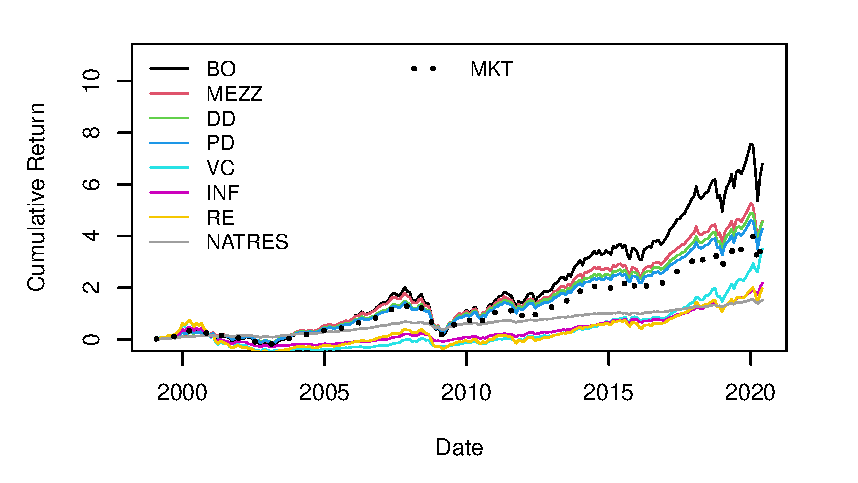
\includegraphics{Figures/Cumulative_Returns_2020.eps}
	\caption{
		PREQIN 2023: Cumulative USD returns implied by the MSCI World factor models from Table \ref{tab:average_coefs_preqin_2020} from 1999-01-31 until 2023-02-28.}
	\label{fig:cum_returns_preqin}   
\end{figure}



% latex table generated in R 3.6.1 by xtable 1.8-4 package
% Tue Jul 28 12:13:36 2020
\begin{table}[ht]
	\centering
	\begin{tabular}{lrrrrrrrr}
		Vintage & BO & DD & INF & MEZZ & NATRES & PD & RE & VC \\ 
		\hline
		\hline
		%1983 &   0 &   0 &   0 &   0 &   0 &   0 &   0 &   0 \\ 
		1984 &   0 &   0 &   0 &   0 &   0 &   0 &   0 &   1 \\ 
		1985 &   3 &   0 &   0 &   0 &   0 &   0 &   0 &   4 \\ 
		1986 &   2 &   0 &   0 &   1 &   0 &   1 &   0 &   4 \\ 
		1987 &   4 &   0 &   0 &   1 &   0 &   1 &   0 &   3 \\ 
		1988 &   7 &   0 &   0 &   0 &   0 &   0 &   0 &   2 \\ 
		1989 &   2 &   0 &   0 &   0 &   1 &   0 &   0 &   2 \\ 
		1990 &   5 &   1 &   0 &   0 &   0 &   1 &   0 &   6 \\ 
		1991 &   3 &   2 &   0 &   0 &   0 &   2 &   0 &   4 \\ 
		1992 &   9 &   2 &   0 &   2 &   1 &   4 &   1 &   7 \\ 
		1993 &   7 &   0 &   0 &   0 &   0 &   0 &   0 &   4 \\ 
		1994 &   9 &   1 &   0 &   2 &   1 &   3 &   1 &   7 \\ 
		1995 &  17 &   0 &   0 &   1 &   1 &   1 &   1 &  10 \\ 
		1996 &  16 &   2 &   0 &   2 &   0 &   4 &   4 &  10 \\ 
		1997 &  16 &   2 &   0 &   0 &   1 &   2 &   6 &  14 \\ 
		1998 &  30 &   1 &   0 &   3 &   2 &   4 &   3 &  23 \\ 
		1999 &  28 &   1 &   0 &   7 &   1 &   8 &   2 &  37 \\ 
		2000 &  32 &   3 &   0 &   4 &   0 &   7 &   6 &  67 \\ 
		2001 &  18 &   2 &   0 &   3 &   1 &   5 &   2 &  40 \\ 
		2002 &  24 &   4 &   1 &   2 &   2 &   6 &   2 &  24 \\ 
		2003 &  18 &   3 &   1 &   2 &   1 &   5 &   6 &  19 \\ 
		2004 &  29 &   2 &   4 &   3 &   2 &   5 &  10 &  29 \\ 
		2005 &  63 &   6 &   0 &   7 &   4 &  14 &  19 &  34 \\ 
		2006 &  76 &  10 &   5 &   5 &   3 &  16 &  34 &  41 \\ 
		2007 &  88 &  13 &   5 &   3 &   7 &  16 &  36 &  53 \\ 
		2008 &  76 &  12 &   3 &   6 &   8 &  21 &  35 &  40 \\ 
		2009 &  35 &   7 &   5 &   4 &   4 &  12 &  14 &  20 \\ 
		2010 &  53 &   9 &   9 &   7 &   8 &  18 &  40 &  21 \\ 
		2011 &  72 &   8 &  11 &   6 &   9 &  16 &  51 &  27 \\ 
		2012 &  69 &  14 &   4 &  11 &  11 &  26 &  42 &  25 \\ 
		2013 &  80 &  15 &  12 &   4 &   8 &  32 &  61 &  30 \\ 
		2014 &  88 &  13 &  12 &   5 &  15 &  31 &  56 &  36 \\ 
		2015 &  99 &  18 &  13 &   7 &   9 &  38 &  86 &  47 \\ 
		2016 & 108 &   8 &  16 &   8 &  16 &  29 &  63 &  56 \\ 
		2017 &  83 &  15 &  20 &   8 &  13 &  48 &  78 &  56 \\ 
		2018 &  88 &  22 &  18 &  11 &   8 &  54 &  71 &  55 \\ 
		2019 &  21 &   3 &   5 &   2 &   1 &  11 &  12 &  11 \\ 
		\hline
		Total & 1378 & 199 & 144 & 127 & 138 & 441 & 742 & 869 \\ 
		\hline
		\hline
	\end{tabular}
	\caption{PREQIN 2020: Number of funds per vintage year in the Preqin dataset used for estimation (Preqin cash flow data set as of 26th February 2020).} 
	\label{tab:preqin_data}
\end{table}


\newpage


% Factor Model Returns + Errors
\renewcommand{\segment}{PE}

\subsection{Preqin: Idiosyncratic returns for \segment \ funds}
\label{sec:preqin_errors_\segment}

\begin{figure}[H]
	\centering
	\includegraphics{Figures/q_factors/XErrorSeries\segment Preqin}
	\caption{Idiosyncratic returns estimated by componentwise $L_2$ boosting for fund type \segment \ in the period from 1990-03-31 until 2019-09-30.}
	\label{fig:preqin_clb_idio_\segment}
\end{figure}

\begin{figure}[H]
	\centering
	\includegraphics{Figures/q_factors/XTotalErrorSeries\segment Preqin}
	\caption{
		Comparison between the total returns for fund type \segment \ implied by our two-factor ensemble and our two-factor ensemble plus the error term from Figure \ref{fig:preqin_clb_idio_\segment}.
		Both series are contrasted against the NAV Return indices provided by Cambridge Associates and Pitchbook and the MSCI stock market index in the period 1990-03-31 until 2019-09-30.
	}
	\label{fig:preqin_clb_total_\segment}
\end{figure}

\begin{figure}[H]
	\centering
	\includegraphics{Figures/q_factors/XTotalErrorSeries\segment Preqinpre2010}
	\includegraphics{Figures/q_factors/XTotalErrorSeries\segment Preqinpost2010}
	\caption{
		In these two subplots, we split the full \segment \ time series from Figure \ref{fig:preqin_clb_total_\segment} into a pre-2010 and post-2010 period.
	}
	\label{fig:preqin_clb_pre_post_2010_\segment}
\end{figure}


% Factor Model Returns + Errors
\renewcommand{\segment}{VC}

\subsection{Preqin: Idiosyncratic returns for \segment \ funds}
\label{sec:preqin_errors_\segment}

\begin{figure}[H]
	\centering
	\includegraphics{Figures/q_factors/XErrorSeries\segment Preqin}
	\caption{Idiosyncratic returns estimated by componentwise $L_2$ boosting for fund type \segment \ in the period from 1990-03-31 until 2019-09-30.}
	\label{fig:preqin_clb_idio_\segment}
\end{figure}

\begin{figure}[H]
	\centering
	\includegraphics{Figures/q_factors/XTotalErrorSeries\segment Preqin}
	\caption{
		Comparison between the total returns for fund type \segment \ implied by our two-factor ensemble and our two-factor ensemble plus the error term from Figure \ref{fig:preqin_clb_idio_\segment}.
		Both series are contrasted against the NAV Return indices provided by Cambridge Associates and Pitchbook and the MSCI stock market index in the period 1990-03-31 until 2019-09-30.
	}
	\label{fig:preqin_clb_total_\segment}
\end{figure}

\begin{figure}[H]
	\centering
	\includegraphics{Figures/q_factors/XTotalErrorSeries\segment Preqinpre2010}
	\includegraphics{Figures/q_factors/XTotalErrorSeries\segment Preqinpost2010}
	\caption{
		In these two subplots, we split the full \segment \ time series from Figure \ref{fig:preqin_clb_total_\segment} into a pre-2010 and post-2010 period.
	}
	\label{fig:preqin_clb_pre_post_2010_\segment}
\end{figure}



% Factor Model Returns + Errors
\renewcommand{\segment}{RE}

\subsection{Preqin: Idiosyncratic returns for \segment \ funds}
\label{sec:preqin_errors_\segment}

\begin{figure}[H]
	\centering
	\includegraphics{Figures/q_factors/XErrorSeries\segment Preqin}
	\caption{Idiosyncratic returns estimated by componentwise $L_2$ boosting for fund type \segment \ in the period from 1992-06-30 until 2019-09-30.}
	\label{fig:preqin_clb_idio_\segment}
\end{figure}

\begin{figure}[H]
	\centering
	\includegraphics{Figures/q_factors/XTotalErrorSeries\segment Preqin}
	\caption{
		Comparison between the total returns for fund type \segment \ implied by our two-factor ensemble and our two-factor ensemble plus the error term from Figure \ref{fig:preqin_clb_idio_\segment}.
		Both series are contrasted against the NAV Return indices provided by Cambridge Associates and Pitchbook and the MSCI stock market index in the period 1990-03-31 until 2019-09-30.
	}
	\label{fig:preqin_clb_total_\segment}
\end{figure}

\begin{figure}[H]
	\centering
	\includegraphics{Figures/q_factors/XTotalErrorSeries\segment Preqinpre2010}
	\includegraphics{Figures/q_factors/XTotalErrorSeries\segment Preqinpost2010}
	\caption{
		In these two subplots, we split the full \segment \ time series from Figure \ref{fig:preqin_clb_total_\segment} into a pre-2010 and post-2010 period.
	}
	\label{fig:preqin_clb_pre_post_2010_\segment}
\end{figure}



\end{document}
